\documentclass[11pt,a4paper]{article}
\usepackage[utf8]{inputenc}
\usepackage[T1]{fontenc}
\usepackage{amsmath, amssymb, amsfonts}
\usepackage{geometry}
\usepackage{graphicx}
\usepackage{booktabs}
\usepackage{hyperref}
\usepackage{enumitem}
\usepackage{pgfplots}
\usepackage{tabularx}
\usepackage{comment}
\usepackage{subcaption}
% Repository holding the implementation referenced in Appendix~\ref{app:code}.
\newcommand{\codeurl}{https://github.com/ZahraAlijani/energy-poverty}

\pgfplotsset{compat=1.18}
\geometry{margin=2.5cm}

\title{Dynamical Modeling of Energy Poverty}
\author{}
\date{}

\begin{document}
\maketitle

\begin{abstract}
Energy poverty is increasingly understood as a multidimensional and dynamic
condition rather than a static state captured by a single affordability
threshold. This paper develops a continuous-time dynamical framework for its
observable dimensions defined on EU--SILC variables: inability to adequately
heat or cool the dwelling, arrears on utility bills, energy burden, and
financial poverty. These dimensions are modeled as continuous deprivation
intensities whose mutual reinforcement and gradual recovery are described by a
linear system admitting closed-form solutions. The analysis identifies the
direct damping of the energy burden as the decisive factor separating a
poverty-trap regime, in which deprivation persists, from a stable regime, in
which it fades regardless of initial conditions. To avoid the artificial
discontinuities of binary indicators, we further introduce a fuzzy extension
that grades deprivation smoothly and aggregates it into a composite fuzzy
energy-poverty index. We illustrate both regimes and the heating and cooling
indicator numerically, and discuss how the stability conditions translate into
structural policy levers such as retrofitting, arrears relief, and energy-burden
reduction. The resulting model is transferable across national
operationalizations and provides an analytically tractable benchmark for
studying the emergence, persistence, and mitigation of energy poverty over time.
\end{abstract}
\section{Conceptualization of Energy Poverty WorldWide}

Energy poverty has increasingly been recognized as a multidimensional and dynamic phenomenon rather than a condition reducible to a single indicator of income or energy expenditure. In general terms, energy poverty refers to a situation in which households are unable to secure adequate energy services necessary for a decent standard of living, including heating, cooling, lighting, cooking, hot water, and the operation of essential household appliances. Such deprivation may result from insufficient income, high energy prices, low energy efficiency of buildings, inadequate infrastructure, or combinations of these factors.

Contemporary research emphasizes that energy poverty extends beyond affordability alone and also includes dimensions of accessibility, reliability, cleanliness, comfort, and the capability to transform energy access into actual wellbeing. In this sense, energy poverty represents not only material deprivation but also a broader limitation of social participation, health, and quality of life.

\subsection{Global Perspectives on Energy Poverty}

The international literature demonstrates substantial geographical variation in the conceptualization and measurement of energy poverty. In high-income economies, research has traditionally focused on affordability-based indicators, particularly expenditure ratios such as the well-known ``10\% rule'' \cite{garcia2019spain,dubois2020france}. However, recent studies criticize fixed expenditure thresholds because they may fail to identify ``hidden energy poverty,'' where households deliberately suppress energy consumption to maintain low expenditures despite inadequate thermal comfort and compromised wellbeing \cite{smith2022hidden,van2021dutchpoverty}.

In contrast, studies conducted in developing regions, including Sub-Saharan Africa, South Asia, and Latin America, typically adopt multidimensional approaches that incorporate access to modern energy infrastructure, reliability, and energy quality. A widely used framework is the Multidimensional Energy Poverty Index (EPI) \cite{nussbaumer2012mepi,patel2021southasia,silva2020latam}. Since physical electrification alone does not guaranty affordable or usable energy services, the EPI evaluates several dimensions of deprivation simultaneously. For households $j$, the index is commonly defined as
\begin{equation}\label{eq:mepi}
EPI_j = \sum_{i=1}^{d} w_i I_{ij},
\end{equation}
where $d$ denotes the number of considered indicators, $w_i$ represents the weight assigned to indicator $i$, and $I_{ij}$ is a binary deprivation indicator for household $j$; see~\cite{moyo2022subsaharan}. Current methodological debates mainly concern the specification of the weights $w_i$, with recent contributions increasingly employing Principal Component Analysis (PCA) instead of equal weighting schemes to reflect regional statistical variability more accurately.

Transitional economies such as China increasingly combine affordability and infrastructural perspectives. Recent studies highlight the importance of clean cooking fuels, winter heating affordability, and environmental sustainability as rural electrification reaches saturation levels \cite{wang2021rural,li2022transitioning}.

\subsection{Social and Demographic Dimensions}

Energy poverty interacts strongly with existing social and demographic vulnerabilities. The literature consistently identifies elderly populations, women, rural households, and low-income groups as particularly exposed.

Older adults are especially vulnerable due to fixed incomes, greater thermoregulatory needs, and increased health sensitivity to inadequate housing conditions. Longitudinal studies associate prolonged exposure to cold indoor environments and biomass pollution with deteriorating physical and mental health, including cognitive decline \cite{muller2021elderly,lee2023cognitive,chen2023aging}.

In many developing regions, energy poverty also exhibits a pronounced gender dimension. Dependence on traditional biomass fuels often generates severe ``time poverty,'' as women spend substantial amounts of time collecting fuel and managing household energy needs. This restricts educational and economic opportunities while simultaneously increasing exposure to harmful indoor air pollution \cite{kaur2021timepoverty,njoku2022gendered,rahman2023disasters}. Natural disasters and environmental shocks may further intensify these vulnerabilities by damaging infrastructure and forcing households to revert to polluting traditional fuels.

\subsection{Dynamic and Temporal Nature of Energy Poverty}

Recent research increasingly emphasizes that energy poverty is not a static condition but a dynamic process characterized by persistence, transitions, and vulnerability to external shocks. Households may experience chronic energy poverty, temporary deprivation, or repeated transitions between vulnerable and non-vulnerable states.

Budr\'ia and Velasco-Gallego \cite{BUDRIA2026104670} identify several distinct trajectories of energy poverty, including persistently non-poor households, temporarily vulnerable households, volatile households, and long-term declining households. Similarly, Masciandaro et al.~\cite{MASCIANDARO2026115318} show that the probability of entering or remaining in energy poverty differs substantially across countries and household types. Chen et al.~\cite{CHEN2026109339} distinguish between chronic and transient forms of energy poverty, highlighting the importance of duration and persistence in both measurement and policy design.

This temporal dimension suggests that energy poverty should not be conceptualized solely as a short-term inability to pay energy bills. Instead, it should also reflect structural vulnerabilities that generate long-term risks of deprivation. These vulnerabilities may include unstable income, poor housing quality, demographic pressures, financial exclusion, regional inequalities, and exposure to geopolitical or environmental shocks \cite{ULLAH2026115185,ALI2026115278}.

\subsection{Policy Perspectives and Structural Interventions}

The current policy-oriented literature increasingly advocates structural rather than purely reactive approaches to energy poverty alleviation. Direct subsidies for energy bills are often criticized as short-term measures that fail to address underlying structural causes such as low building efficiency and poor housing conditions \cite{perez2023retro,jansen2022subsidies}.

Consequently, many studies emphasize long-term interventions, including residential retrofits, energy-efficient renovations, modernization of heating systems, and improved financial inclusion \cite{zhang2022fintech,okocha2023mobilemoney}. Digital financial tools and broader access to credit may improve households' ability to invest in cleaner and more efficient energy technologies.

At the same time, the literature warns about unintended policy consequences. For example, strict environmental regulations without adequate compensatory mechanisms may deepen energy vulnerability among low-income rural populations \cite{liu2021straw,zhao2022unintended}. Effective policy design, therefore, requires integrated approaches that combine environmental objectives, social protection, housing policy, and infrastructure development \cite{kone2023sez}.

%%%%%%%%%%%%%%%%%%%%%%%%%%%%%%%%%%%%%%%%%%%%%%%%%%%%%%%%
\section{Motivation for a Dynamical Perspective and Graduality of Energy Poverty}

Energy poverty exhibits substantial persistence and delayed responses to economic, infrastructural, and policy-related shocks. However, the development of empirically validated dynamical models is often constrained by limited longitudinal data availability. In many contexts, sufficiently long and reliable time series do not yet exist, making purely data-driven long-term forecasting difficult.

Nevertheless, the absence of long historical datasets does not invalidate a dynamical approach. A theoretical dynamical framework remains valuable because it formalizes the structural relationships among income, energy expenditures, arrears, housing efficiency, and external policy interventions. Such models make it possible to distinguish between short-term responses, long-run equilibria, transitional dynamics, and feedback effects that cannot easily be captured by static statistical approaches.

An additional advantage of the proposed framework is its analytical tractability. Because the system admits explicit mathematical analysis, one can directly study equilibria, stability properties, adjustment speeds, and parameter sensitivities without relying exclusively on extensive empirical calibration. The primary purpose of the present framework is therefore not immediate forecasting accuracy, but rather the construction of a coherent theoretical benchmark that clarifies the mechanisms underlying energy poverty dynamics and provides a basis for future empirical refinement.

\subsection{Indicators for Energy Poverty Dynamics}

Within the European Union, energy poverty is generally understood as a situation in which households are forced to reduce energy consumption to a level that negatively affects health and wellbeing. According to the European Commission, the principal drivers of energy poverty include low household income, high energy prices, and poor energy performance of buildings and appliances.

The European approach also recognizes the growing importance of ``summer energy poverty,'' referring to the inability to maintain safe indoor temperatures during heat waves. This issue has become increasingly relevant in the context of climate change and urban overheating.

Following the COVID-19 crisis, rising energy prices, and geopolitical instability associated with the Russian invasion of Ukraine, energy poverty became a central policy concern across Europe. In response, the EU introduced multiple instruments, including the Social Climate Fund, revised directives on energy efficiency and electricity markets, and the Energy Poverty Advisory Hub, which provides technical assistance and methodological support to local authorities.

As an example, let us mention that in 2025, the Czech Ministry of Industry and Trade formally adopted a national definition of energy poverty following consultations with an expert working group composed of representatives from academia, public administration, and other stakeholders, see~\cite{mpo2025_definition,klusacek_kalenda2024_energypoverty}. It is operationalized using household-level indicators available in the EU-SILC database. In this framework, energy poverty is conceptualized as a multidimensional condition reflecting insufficient access to socially necessary energy services at an affordable cost, and it employs three complementary indicators:
\begin{itemize}
    \item[\textbf{I1:}] inability to adequately heat or cool the dwelling,
    \item[\textbf{I2:}] arrears on utility or energy payments,
    \item[\textbf{I3:}] simultaneous occurrence of high energy expenditure burden and income poverty.
\end{itemize}
These indicators capture complementary dimensions of energy vulnerability, including subjective thermal deprivation, financial stress, and objective expenditure burden.

The use of these three indicators is therefore not intended to reduce energy poverty to three isolated symptoms, but to provide a parsimonious operational representation of its main mechanisms within the dynamical system. Each indicator corresponds to a different channel through which energy poverty evolves: inadequate heating reflects unmet energy needs, arrears capture the accumulation of financial pressure, and high energy burden represents the structural imbalance between household resources and energy costs. Together, they allow the model to distinguish between deprivation, debt formation, and affordability constraints. This is important because households may enter energy poverty through different pathways, and the same prevalence level may correspond to different underlying dynamics. 

At the same time, the proposed framework is not tied exclusively to the Czech operationalization. In another national context, the three indicators may be replaced by locally relevant measures, such as lack of access to clean cooking fuels, unreliable electricity supply, inability to cool the dwelling, or dependence on traditional biomass. The structure of the dynamical system remains unchanged, while the empirical meaning of its components is adapted to the institutional, climatic, and socio-economic conditions of the country under study. Thus, the model should be understood as a transferable framework: national indicators define how energy poverty is observed, whereas the dynamical system describes how its main dimensions interact and evolve over time.

\subsection{From Binary Classification to Gradual Energy Poverty Indices}

A substantial limitation of many traditional approaches to energy poverty measurement is the reliance on binary classification schemes. In such frameworks, households are typically classified as either energy poor or non-energy poor according to fixed thresholds. For example, whether energy expenditures exceed a predefined proportion of income or whether a household reports an inability to adequately heat the dwelling; e.g., if $I_1, I_2,I_3$ is defined as binary, then usually energy poverty is defined as $I_1(x)\vee I_2(x)\vee I_3(x)$ for a household $x$, hence, also binary. Although these indicators are easy to interpret and operationalize, they introduce an artificial discontinuity into a phenomenon that is inherently gradual and multidimensional.

In reality, energy vulnerability rarely emerges abruptly at a single threshold value. Households located just below and just above a predefined cutoff are often socio-economically very similar, yet binary indicators assign them completely different statuses. This may lead to loss of information, reduced sensitivity to moderate vulnerability, and instability of empirical conclusions under small variations in income, prices, or weather conditions. Furthermore, binary indicators are unable to adequately capture partial deprivation, cumulative disadvantage, or varying intensities of exposure across households.

For these reasons, recent research increasingly emphasizes the importance of gradual and continuous representations of energy poverty. Fuzzy logic provides a natural mathematical framework for such an extension because it allows households to belong to the set of energy-poor households only to a certain degree rather than absolutely. Instead of binary deprivation indicators taking values only in $\{0,1\}$, fuzzy indicators take values in the interval $[0,1]$, where higher values represent higher intensity of deprivation.

Under this approach, each household $x$ is characterized by fuzzy indicator degrees
\[
\tilde I_{i}(x) \in [0,1],
\]
where $\tilde I_{i}(x)$ expresses the degree to which household $x$ is deprived in dimension $i$. The multidimensional energy poverty index can then be generalized to the gradual form as
\begin{equation}
\label{eq:fuzzy_mepi}
\tilde P(x) = \bigoplus_{i=1}^{d} \tilde I_{i}(x),
\end{equation}
and possibly with weights expressing importance of the particular indicator
\begin{equation}
\label{eq:fuzzy_mepi}
\tilde P_w(x) = \bigoplus_{i=1}^{d} (w_i\otimes \tilde I_{i}(x)),
\end{equation}
where $\oplus$ is a generalization of classical disjunction $\vee$, $\otimes$ is a generalization of classical conjunction $\wedge$ and $\tilde I_{i}(x)$ represents the degree of deprivation instead of a binary indicator. The classical binary formulation becomes a special case obtained when all $\tilde I_{i}(x)$ attain only values $0$ or $1$.

This gradual formulation provides several advantages. First, it preserves substantially more information about the intensity and structure of household vulnerability. Second, it reduces instability caused by arbitrary threshold effects. Third, it enables smoother integration with dynamical models, where abrupt discontinuities may create unrealistic transitions and analytical difficulties. In particular, continuous fuzzy indicators are more suitable for studying persistence, trajectories, and nonlinear feedback mechanisms in energy poverty dynamics. Finally, fuzzy formulations better reflect the social-science interpretation of deprivation as a continuum rather than a strictly dichotomous state.

Consequently, introducing fuzzy logic into multidimensional energy poverty measurement represents not merely a technical modification, but a conceptual shift from categorical classification toward gradual vulnerability assessment. Such an approach is especially relevant when energy poverty is analyzed as a dynamic and evolving process influenced by interacting economic, infrastructural, demographic, and environmental factors.

Note: weights can be present as well.

\subsection{Gradual Energy Poverty in a Dynamical Framework}

The transition from binary to gradual representations of energy poverty is particularly important when energy poverty is studied as a dynamical phenomenon. Binary indicators are suitable for static classification, but they become problematic in dynamical systems because they introduce abrupt discontinuities into the evolution of household states. In reality, however, households typically move into and out of energy poverty gradually through cumulative economic pressure, changing energy prices, deteriorating housing conditions, or progressive indebtedness. A continuous representation is therefore substantially more consistent with the temporal and structural nature of energy vulnerability.

The incorporation of fuzzy logic into the dynamical framework allows energy poverty to be modeled as a continuously evolving degree of vulnerability rather than as a discrete state transition. Instead of assuming that households instantaneously switch from ``non-poor'' to ``energy poor'' after crossing an arbitrary threshold, fuzzy indicators permit smooth transitions reflecting varying intensities of deprivation. This is especially relevant for households located near conventional cut-off values, where small fluctuations in income, weather conditions, or energy expenditures may otherwise produce unrealistic jumps between states.

Within this framework, the dynamical system no longer describes only the evolution of observable economic variables, but also the gradual propagation of deprivation across multiple dimensions. For example, increasing energy prices may initially increase the energy burden component, which subsequently contributes to arrears accumulation and eventually to inadequate heating conditions. Similarly, investments into housing renovation may progressively reduce deprivation intensity instead of causing an instantaneous transition from energy poverty to non-poverty.

An important advantage of this formulation is that the resulting trajectories become smoother and analytically more tractable. Continuous fuzzy indicators naturally integrate with differential or difference equation systems and allow the analysis of persistence, stability, feedback loops, and tipping effects without introducing unrealistic discontinuities. Moreover, the framework permits the modeling of partial policy effects. For instance, a subsidy or renovation program may reduce the degree of vulnerability even if it does not fully eliminate energy poverty according to a binary definition.

The gradual dynamical perspective also improves comparability across countries and institutional settings. Different national operationalizations may employ different deprivation indicators, thresholds, or weighting schemes, while the underlying dynamical structure remains conceptually unchanged. The model therefore separates two levels of analysis: the empirical specification of deprivation dimensions and the general mechanisms governing their interaction and temporal evolution.

From this perspective, energy poverty should not be interpreted as a fixed categorical status, but rather as a continuously evolving state of household vulnerability generated by interacting economic, infrastructural, demographic, and environmental processes. The integration of fuzzy logic with dynamical systems thus provides a mathematically flexible and socially realistic framework for studying the emergence, persistence, and mitigation of energy poverty over time.
\section{Methods used in modeling energy poverty}

Energy poverty has emerged as a major barrier to global sustainable development, representing the inability of households to access adequate, reliable, and affordable energy for essential daily needs such as heating, cooling, and lighting. To comprehensively understand and address the multifaceted nature of energy poverty, the academic literature has increasingly deployed a highly diverse and sophisticated range of methodological approaches. These methods span from multidimensional index construction and causal econometric modeling to advanced spatial analyses, artificial intelligence, and systems thinking.


%%%%%%%%%%%%%%%%%%%%%%%%%%%%%%%%%%

\begin{table}[h!]
\centering
\scriptsize
\begin{tabular}{p{3.3cm} p{8.5cm}}
\toprule
\textbf{Category} & \textbf{Methods and References} \\
\midrule

\textbf{Measurement \& Indices} 
& 10\% Rule, LIHC (affordability thresholds) \\
& \cite{FENG2026107062, CRETI2026109209, ADABOR2026115293, 
dubois2020france, garcia2019spain, van2021dutchpoverty} \\

& MEPI (Alkire--Foster multidimensional index) \\
& \cite{nussbaumer2012mepi, MAHMOOD2026102127, XU2026109217} \\

& PCA-based weighting (data-driven index construction) \\
& \cite{GONG2026115104, yang2026multidimensional, XIE2026109295,
moyo2022subsaharan, silva2020latam, patel2021southasia} \\

& FGT-type indices (structural vs transient poverty) \\
& \cite{CHEN2026109339, rahman2023disasters} \\

& Hidden energy poverty (self-rationing) \\
& \cite{WHITE2026104583, smith2022hidden} \\

\midrule

\textbf{Econometric Models} 
& TWFE and IV models (causal estimation) \\
& \cite{ULLAH2026115185, zhou2026graying, ADABOR2026115293} \\

& DID approaches (policy evaluation) \\
& \cite{XU2026109217, liu2021straw, wang2021rural, zhao2022unintended} \\

& Policy and financial inclusion studies \\
& \cite{jansen2022subsidies, perez2023retro, ADJEIMANTEY2026140083,
okocha2023mobilemoney, zhang2022fintech} \\

\midrule

\textbf{Spatial Analysis} 
& ESTDA, SDM, GWR (spatial heterogeneity and spillovers) \\
& \cite{XIE2026109295, yang2026multidimensional} \\

& Infrastructure and regional development (SEZ, micro-grids) \\
& \cite{GONG2026115104, kone2023sez} \\

\midrule

\textbf{Machine Learning} 
& DTW, 1D-CNN (dynamic trajectories) \\
& \cite{BUDRIA2026104670} \\

& Clustering (household vulnerability profiles) \\
& \cite{CRETI2026109209, kaur2021timepoverty, njoku2022gendered} \\

& Demographic/aging analysis \\
& \cite{taylor2020pension, muller2021elderly, li2022transitioning} \\

\midrule

\textbf{Systems Modeling} 
& System Dynamics (feedback systems) \\
& \cite{ZARGHAMI2026127902} \\

& GSEM and causal mediation \\
& \cite{ULLAH2026115185, ADABOR2026115293} \\

& Health and cognitive impacts \\
& \cite{chen2023aging, lee2023cognitive} \\

\bottomrule
\end{tabular}
\caption{Overview of methodological approaches in energy poverty research.}
\label{tab:methods}
\end{table}

%%%%%%%%%%%%%%%%%%%%%%%%%%%%%%%%%%%%%%%%%%%%%%%%%%%%%%%%%%%%5
\begin{table}[h!]
\centering
\begin{tabular}{ll}
\toprule
Symbol & Meaning \\
\midrule
$h(t)$ &  Convenient temperature \\
$b(t)$ & Energy burden \\
$d(t)$ & Energy-related debts \\
$p(t)$ & Financial poverty \\
\midrule
$I_1,I_2,I_3$ & Binary EU--SILC indicators \\
$\tau_b$ & Burden thresholds \\
$\tau_c$ & Cooling thresholds \\
$\tau_d$ & Debt  thresholds \\
$\tau_p$ & Poverty thresholds \\
$\tilde I_1,\tilde I_2,\tilde I_3$ & Fuzzy indicators \\
$\tilde P$ & Fuzzy energy poverty \\
$L_b,U_b$ & Fuzzy burden thresholds \\
$L_h,U_h$ & Fuzzy heating thresholds \\
$L_c,U_c$ & Fuzzy cooling thresholds \\
$L_d,U_d$ & Fuzzy debt thresholds \\
$L_p,U_p$ & Fuzzy poverty thresholds \\







\midrule
$\otimes$ & Product t-norm: $x\otimes y = xy$ \\
$\oplus$ & T-conorm (probabilistic sum) \\
$\Psi_{0\to 1}$ & Increasing cosine ramp \\
$\Psi_{1\to 0}$ & Decreasing cosine ramp \\
\bottomrule
\end{tabular}
\caption{Overview of symbols in use.}\label{tab:symbols}
\end{table}

%%%%%%%%%%%%%%%%%%%%%%%%%%%%%%%%%%%%%%%%%%%%%%%%%%%new simplified model
\section{ Dynamical Representation Based Only on EU--SILC Variables}
\subsection{Introduction to the Model}

The following model is designed to describe the dynamics of the main observable dimensions entering the definition of energy poverty, rather than the dynamics of the composite energy-poverty indicator itself. In particular, it focuses on the temporal evolution of inability to heat the dwelling adequately, arrears on utility bills, energy burden, and poverty status. These quantities are interpreted as continuous intensity variables derived from EU--SILC indicators.

This approach is appropriate because the composite energy-poverty status is defined only as a logical combination of these dimensions, whereas the dimensions themselves may display persistence and mutual interactions over time. The purpose of the model is therefore to capture how changes in one dimension may affect the others and how adverse conditions may accumulate or gradually diminish. The resulting framework provides a simplified-form dynamical representation of the observable components underlying energy poverty.
If the model is required to rely only on variables directly observed in EU--SILC or constructed from them, then a simplified-form dynamical representation is more appropriate than the mechanistic system based on latent technical quantities. In that case, the state is defined directly in terms of the observable dimensions of energy poverty.

Let
\[
\dot{x}(t) = f(x(t)), 
\qquad 
x(t)=
\begin{bmatrix}
h(t)\\
d(t)\\
b(t)\\
p(t)
\end{bmatrix}\in[0,1]^4,
\]
where \(h(t)\) denotes inability to heat or cool the dwelling adequately, \(d(t)\) arrears on utility bills, \(b(t)\) the energy-burden component, and \(p(t)\) the financial poverty component. All these quantities are either directly observed in EU--SILC or they can be constructed from EU--SILC variables.

% Throughout the simplified-model sections, $p(t)$ denotes the poverty component,
% while $\tilde p(t)$ denotes the composite fuzzy energy poverty index.

\paragraph{State-space invariance.}
The simplified system is defined on the compact state space $[0,1]^4$. Under
nonnegative coefficients and $\lambda_i>0$, the hypercube $[0,1]^4$ is forward
invariant. That is, if $x(0)\in[0,1]^4$, then $x(t)\in[0,1]^4$ for all $t\ge0$,
provided that trajectories are interpreted as intensities truncated at the
boundaries.

This guarantees that the model respects the natural bounds of indicator-based
variables and prevents economically meaningless states.

A simple continuous-time simplified system can be written as
\begin{align}
\dot{h}(t) &= \alpha_1 b(t)+\beta_1 p(t)-\lambda_1 h(t),\\
\dot{d}(t) &= \alpha_2 b(t)+\beta_2 p(t)-\lambda_2 d(t),\\
\dot{b}(t) &= \alpha_3 b(t)+\beta_3 p(t)+\gamma_3 d(t)-\lambda_3 b(t),\\
\dot{p}(t) &= \alpha_4 p(t)+\beta_4 d(t)+\gamma_4 h(t)-\lambda_4 p(t),
\end{align}
where all coefficients are nonnegative. This system represents mutual reinforcement between the observable dimensions of deprivation while avoiding the introduction of latent variables such as technical efficiency or physical energy need.

Or equivalently, a simple continuous-time simplified system may be formulated as
\begin{align}
\dot{h}(t) &= -\lambda_h h(t) + \alpha_{hb} b(t) + \alpha_{hp} p(t),\\
\dot{d}(t) &= -\lambda_d d(t) + \alpha_{db} b(t) + \alpha_{dp} p(t),\\
\dot{b}(t) &= -\lambda_b b(t) + \alpha_{bd} d(t) + \alpha_{bp} p(t),\\
\dot{p}(t) &= -\lambda_p p(t) + \alpha_{pd} d(t) + \alpha_{ph} h(t),
\end{align}
where each diagonal term \(-\lambda_i x_i(t)\) captures the tendency of the corresponding dimension to decrease in the absence of reinforcing factors, and the off-diagonal terms represent cross-effects between the observed dimensions of deprivation.
\subsection{Interpretation and Justification of the Simplified Dynamic Representation}

The simplified system
\begin{align}
\dot{h}(t) &= -\lambda_h h(t) + \alpha_{hb} b(t) + \alpha_{hp} p(t), \label{eq:red_h}\\
\dot{d}(t) &= -\lambda_d d(t) + \alpha_{db} b(t) + \alpha_{dp} p(t), \label{eq:red_d}\\
\dot{b}(t) &= -\lambda_b b(t) + \alpha_{bd} d(t) + \alpha_{bp} p(t), \label{eq:red_b}\\
\dot{p}(t) &= -\lambda_p p(t) + \alpha_{pd} d(t) + \alpha_{ph} h(t) \label{eq:red_p}
\end{align}
is intended as a simplified-form dynamical representation of the main observable dimensions of energy poverty. Here,
\(h(t)\) denotes inability to heat the dwelling adequately,
\(d(t)\) arrears on utility bills,
\(b(t)\) the energy-burden component,
and \(p(t)\) the poverty component.
All four variables are interpreted either as binary indicators smoothed to the interval \([0,1]\), or as continuous intensity scores derived from EU--SILC variables.

The diagonal terms \(-\lambda_h h(t)\), \(-\lambda_d d(t)\), \(-\lambda_b b(t)\), and \(-\lambda_p p(t)\), with \(\lambda_h,\lambda_d,\lambda_b,\lambda_p>0\), represent the natural tendency of each deprivation dimension to decrease in the absence of reinforcing pressures. In substantive terms, these coefficients capture recovery, adaptation, or exit from the corresponding adverse state. Without such terms, the system would contain only amplification mechanisms and would therefore lack a stabilizing force.

The off-diagonal terms represent cross-effects between the dimensions. In particular, the term
\(\alpha_{hb} b(t)\) expresses the idea that a high energy burden increases the risk of inadequate heating, since households facing disproportionately high energy costs may reduce consumption below adequate thermal comfort. The term \(\alpha_{hp} p(t)\) reflects the fact that poverty further limits the ability to maintain adequate heating conditions.

Similarly, the equation for \(d(t)\) states that arrears are more likely when the household faces a high energy burden or is poor. The coefficient \(\alpha_{db}\) captures the mechanism that high energy expenditure relative to available resources increases the probability of falling behind on utility payments, while \(\alpha_{dp}\) reflects the broader financial fragility associated with poverty.

The dynamics of \(b(t)\) are influenced by \(d(t)\) and \(p(t)\). The term \(\alpha_{bd} d(t)\) expresses that households already in arrears are likely to experience persistent affordability stress, while \(\alpha_{bp} p(t)\) captures the empirical fact that poverty is strongly associated with excessive relative energy expenditure.

Finally, the poverty component \(p(t)\) is reinforced by both arrears and heating deprivation. The term \(\alpha_{pd} d(t)\) reflects the fact that payment difficulties are a manifestation of deeper material hardship, whereas \(\alpha_{ph} h(t)\) captures the close link between inability to afford adequate heating and broader poverty or deprivation.

The system is therefore not meant to describe the physical or engineering mechanisms of household energy use. Rather, it is a simplified-form representation of mutual reinforcement among the observed dimensions entering the definition of energy poverty. Its purpose is to capture the qualitative feedback structure:
\[
\text{poverty} \;\longleftrightarrow\; \text{energy burden} \;\longleftrightarrow\; \text{arrears},
\qquad
\text{poverty} \;\longleftrightarrow\; \text{inability to heat adequately}.
\]
This interpretation is consistent with the indicator-based definition of energy poverty, according to which a household is energy poor if it experiences at least one of the following conditions: inability to heat the dwelling adequately, arrears on utility bills, or the joint occurrence of high energy burden and poverty.

A further justification of \eqref{eq:red_h}--\eqref{eq:red_p} is methodological. If the model is required to rely only on quantities observed in EU--SILC or directly constructed from them, then it is preferable to avoid latent variables such as technical efficiency, physical energy need, or investment flows. The simplified system achieves this by operating directly on the observable deprivation dimensions themselves. It should therefore be understood as a parsimonious empirical abstraction rather than a fully structural model of household behavior.

In summary, the proposed representation is justified on three grounds. First, it respects the data constraint by using only EU--SILC-based dimensions. Second, it reflects the empirically plausible mutual reinforcement among heating inadequacy, arrears, energy burden, and poverty. Third, the decay terms ensure that the system has a meaningful interpretation as a dynamic process with both persistence and potential recovery.

\subsection{Energy Poverty Indicators}
In the following, we will use thresholding instead of concrete values because each country computes energy poverty using a different approach. Unlike our Czech threshold of 20\% of income spent on energy, many European approaches do not rely on a single absolute cutoff. A widely used EU expenditure-based indicator is the “2M” measure, which identifies households whose energy expenditure share exceeds twice the national median, while some countries use fixed 10\% rules and others rely on multidimensional indicator sets~\cite{EPAH_indicators_dashboard}. The binary indicators are then defined by thresholding:
\begin{align} \label{binary indicators new}
I_1(t) &= \mathbf{1}\{(h(t)\leq \tau_0)\vee(h(t)\geq\tau_1)\},\\
I_2(t) &= \mathbf{1}\{d(t)\ge \tau_2\},\\
I_3(t) &= \mathbf{1}\{b(t)\ge \tau_3 \land \underbrace{\textsc{Income}(t)\leq \tau_4}_{
  \substack{\text{financial poverty}\\{p(t)}}
}\},
\end{align}
and the final energy-poverty status is
\[
E_P(t)=\mathbf{1}\{I_1(t)\lor I_2(t)\lor I_3(t)\}.
\]

\subsection{Analytical Solutions}\label{Analytical Solutions}
The simplified system can be written in matrix form as
\[
\dot{x}(t)=Ax(t),
\qquad
x(t)=
\begin{bmatrix}
h(t)\\ d(t)\\ b(t)\\ p(t)
\end{bmatrix},
\]
with
\[
A=
\begin{bmatrix}
-\lambda_h & 0 & \alpha_{hb} & \alpha_{hp}\\
0 & -\lambda_d & \alpha_{db} & \alpha_{dp}\\
0 & \alpha_{bd} & -\lambda_b & \alpha_{bp}\\
\alpha_{ph} & \alpha_{pd} & 0 & -\lambda_p
\end{bmatrix}.
\]




\paragraph{Monotonicity.}
The simplified system belongs to the class of cooperative (monotone) dynamical
systems. All off-diagonal entries of $A$ are nonnegative, hence $A$ is a Metzler
matrix. Consequently, the flow generated by $\dot x = Ax$ is order-preserving:
if $x(0)\le y(0)$ componentwise, then $x(t)\le y(t)$ for all $t\ge0$.

This property implies that larger initial deprivation states cannot evolve into
smaller ones faster than initially better-off states, reinforcing the
interpretability of the dynamics in social terms.
For the initial condition
\[
x(0)=x_0=
\begin{bmatrix}
h_0\\ d_0\\ b_0\\ p_0
\end{bmatrix},
\]
the unique solution is given by
\[
x(t)=e^{At}x_0,
\]
where \(e^{At}\) denotes the matrix exponential. 
The solution has an exponential form because the system is linear with constant coefficients. In the scalar case, the equation
\[
\dot{x}(t)=\lambda x(t)
\]
has the solution \(x(t)=Ce^{\lambda t}\), since the exponential function is characterized by the property that its derivative is proportional to itself. In the vector case,
\[
\dot{x}(t)=Ax(t),
\]
The analogous object is the matrix exponential, and the solution is therefore given by
\[
x(t)=e^{At}x_0.
\]
Indeed, the matrix exponential satisfies
\[
\frac{d}{dt}e^{At}=Ae^{At},
\]
which implies
\[
\frac{d}{dt}\bigl(e^{At}x_0\bigr)=Ae^{At}x_0=Ax(t).
\]

If \(A\) is diagonalizable, i.e.
\[
A=V\Lambda V^{-1},
\qquad
\Lambda=\operatorname{diag}(r_1,r_2,r_3,r_4),
\]
then
\[
x(t)=V e^{\Lambda t} V^{-1}x_0,
\qquad
e^{\Lambda t}=\operatorname{diag}(e^{r_1 t},e^{r_2 t},e^{r_3 t},e^{r_4 t}).
\]
Hence each component of the solution is a linear combination of exponential terms determined by the eigenvalues of \(A\).

\subsection{Equilibria of the Simplified System}

To express the equilibrium of the simplified system in the form introduced in Section \ref{Analytical Solutions}, we define an equilibrium \(x^*=(h^*,d^*,b^*,p^*)^\top\) by the condition
\[
Ax^*=0,
\]
that is,
\begin{align}
0 &= -\lambda_h h^* + \alpha_{hb} b^* + \alpha_{hp} p^*,\\
0 &= -\lambda_d d^* + \alpha_{db} b^* + \alpha_{dp} p^*,\\
0 &= -\lambda_b b^* + \alpha_{bd} d^* + \alpha_{bp} p^*,\\
0 &= -\lambda_p p^* + \alpha_{pd} d^* + \alpha_{ph} h^*.
\end{align}

The trivial equilibrium
\[
x^*=\mathbf{0}
\]
always exists. Moreover, if \(\det(A)\neq 0\), then this is the unique equilibrium. Nonzero equilibria exist only in the singular case \(\det(A)=0\), in which case the equilibrium set is the kernel of \(A\).

The stability of the zero equilibrium is determined by the eigenvalues of \(A\). In particular, \(x^*=\mathbf{0}\) is asymptotically stable if all eigenvalues of \(A\) have negative real parts. A sufficient condition for this is strict diagonal dominance by rows, namely
\begin{align}
\lambda_h &> \alpha_{hb}+\alpha_{hp},\\
\lambda_d &> \alpha_{db}+\alpha_{dp},\\
\lambda_b &> \alpha_{bd}+\alpha_{bp},\\
\lambda_p &> \alpha_{pd}+\alpha_{ph}.
\end{align}
Under these inequalities, the decay effects dominate the reinforcing cross-effects, and all trajectories converge to the origin. It means that the self-damping effect in each equation is stronger than the total reinforcing influence of the remaining variables. Consequently, the feedback interactions are not strong enough to sustain a nonzero state, and all trajectories converge to the zero equilibrium. It translates into policy language as follows: energy poverty can be eradicated only if every mechanism that generates it is counteracted more strongly than it is reproduced by the rest of the social-energy system.

In practical terms, the stability inequalities mean that a society can eliminate energy poverty only if the direct corrective mechanisms in each dimension are stronger than the reinforcing spillovers coming from the remaining dimensions. Thus, policies must not only reduce individual manifestations of energy poverty, such as inadequate heating, arrears, or excessive energy burdens, but also weaken the feedback channels through which these problems reproduce one another. A stable zero equilibrium, therefore, corresponds to a policy regime in which housing efficiency, income protection, debt management, and affordability measures jointly dominate the systemic forces generating energy deprivation.
%%%%%%%%%%%%%%%%%%%%%%%%%%%%%%%%%%%%%%%%%%%%%%%%%%%%%%%%%%%%%%%%%%%%%
\subsection{Illustrative Dynamic Simulations}\label{sec:sim}
{\color{red} Martina, I invited you to GitHub, please check your email.}
All codes used in the simulations below are available in the repository
\url{\codeurl}; 
%an interactive version is also provided at
%\url{https://colab.research.google.com/drive/1BPsg4uu6w58Y-TCjLL7HY42we5hLK4HZ?usp=sharing}.
All figures of this paper are produced from the model itself by the script
\texttt{paper\_figures.py}, which integrates the system, evaluates the fuzzy
indicators, and reports the eigenvalues and index levels quoted in the text; see
Appendix~\ref{app:code} and Table~\ref{tab:code-map} for the correspondence
between the figures and the code.

While the analytical results characterize stability and persistence in terms of
eigenvalues and parameter inequalities, it is useful to illustrate the
qualitative implications of these results by means of numerical simulations.
The simulations presented below are intended to demonstrate typical dynamic
patterns of the simplified system under different parameter regimes rather than
to provide empirical calibration or forecasting.

\subsubsection{Poverty-Trap Regime without Direct Energy-Burden Self Correction}\label{sec:sim-trap}

We first consider a parameter configuration in which heating inadequacy,
arrears, and poverty exhibit intrinsic recovery, while the energy-burden
dimension lacks direct self-correction. Formally, this corresponds to
$\lambda_h>0$, $\lambda_d>0$, $\lambda_p>0$, and $\lambda_b=0$.

This configuration represents a situation in which affordability pressures are
not structurally corrected, but persist through reinforcing feedback from
arrears and poverty. Such a regime may reflect policy environments relying
primarily on temporary subsidies or income transfers without addressing the
underlying drivers of high relative energy costs.

\begin{figure}[h!]
\centering
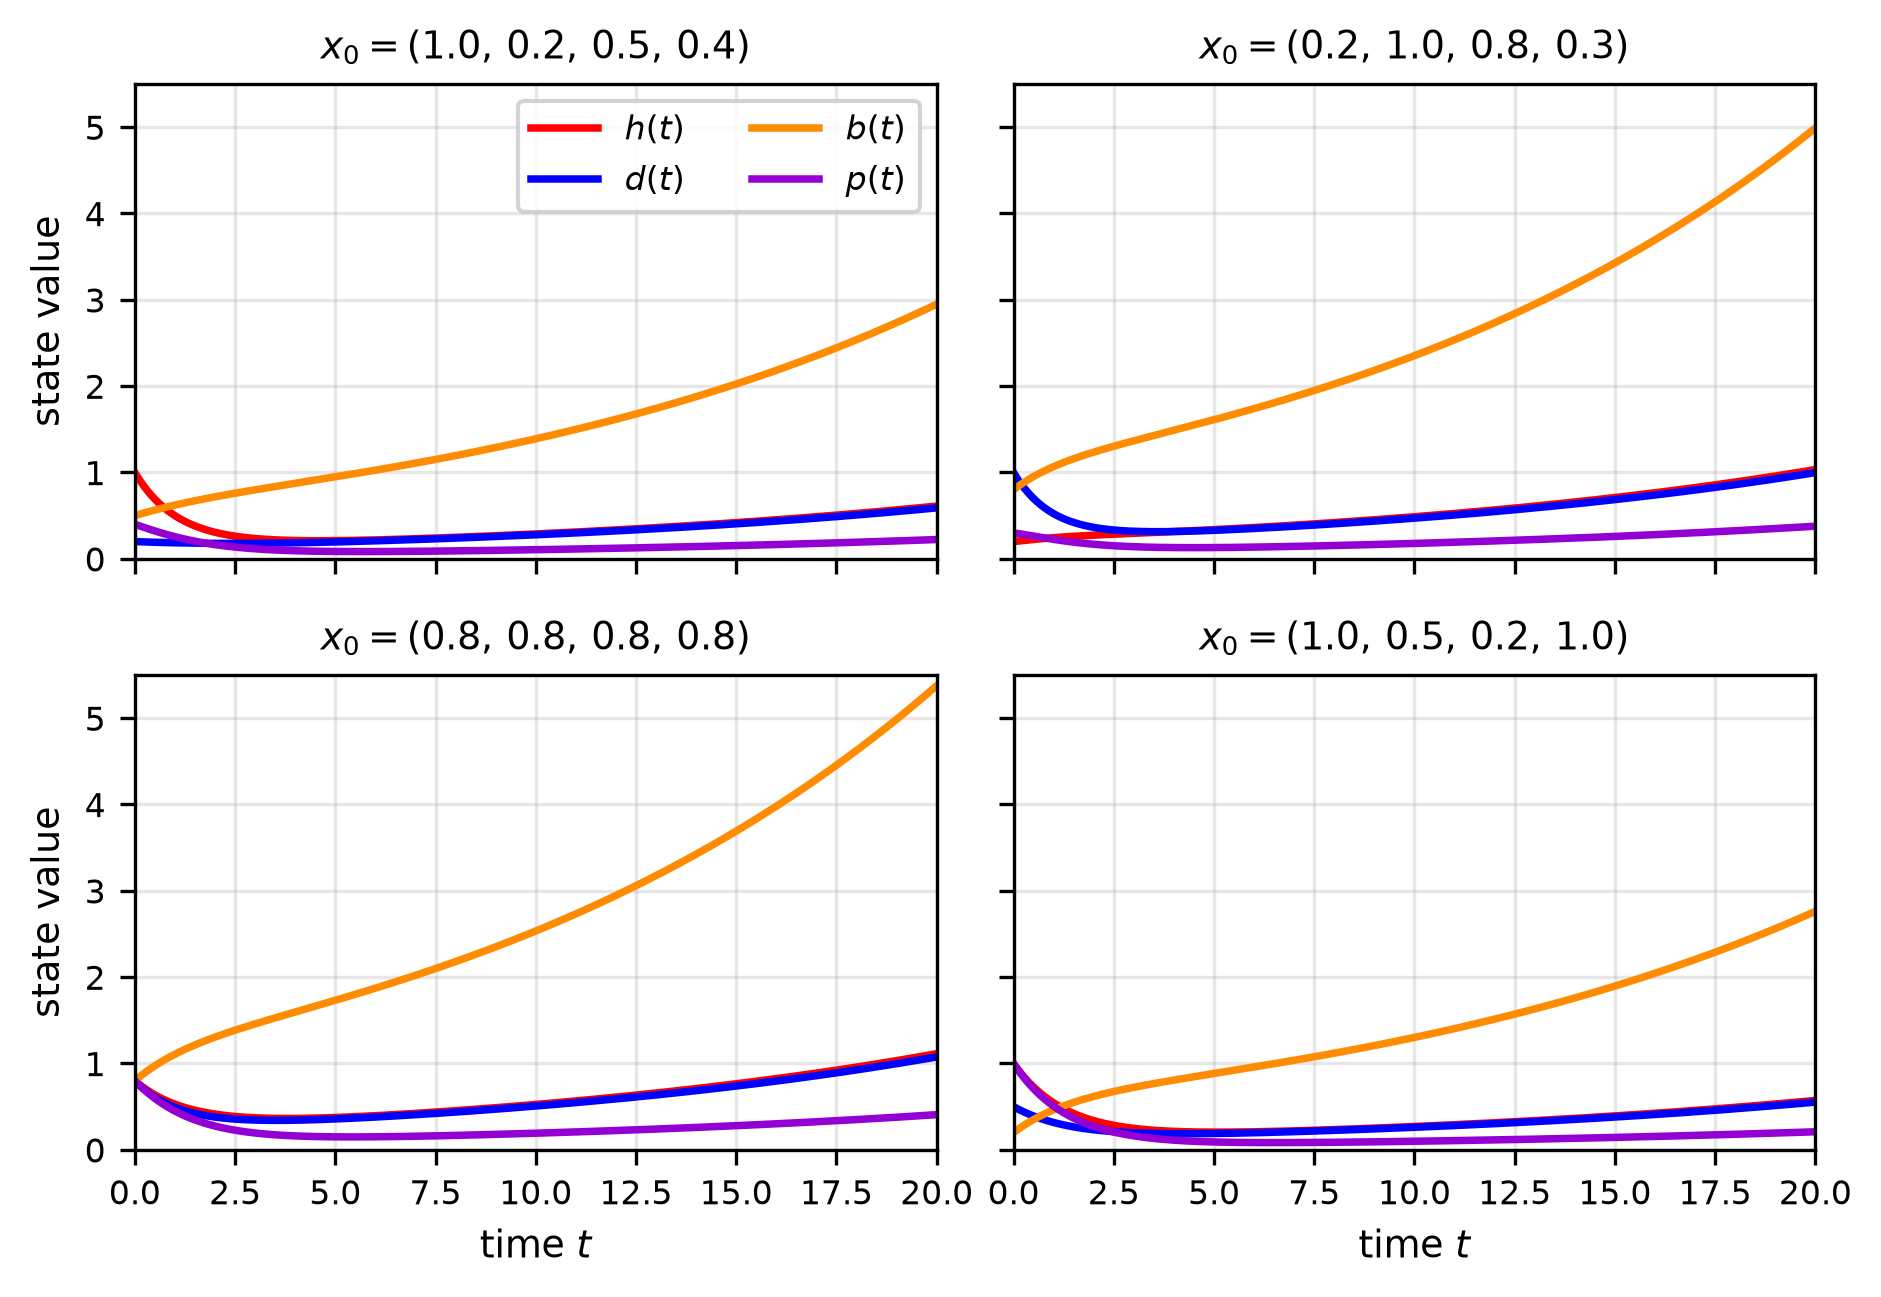
\includegraphics[width=\textwidth]{img/fig1_trap_trajectories.png}
\caption{Multi-panel simulation of the simplified energy poverty dynamics in a
poverty-trap regime ($\lambda_b=0$, $\lambda_h=\lambda_d=\lambda_p=1$). Each
panel corresponds to a different initial condition and shows the time evolution
of inability to heat the dwelling $h(t)$, arrears $d(t)$, energy burden $b(t)$,
and poverty $p(t)$. Since $\lambda_b=0$, the invariance of $[0,1]^4$ is not
guaranteed in this regime; values of the energy burden above one are plotted as
generated by the linear system and correspond, under the intensity
interpretation, to a state truncated at the upper boundary.}
\label{fig:unstable}
\end{figure}

The eigenvalues of the system matrix in this regime consist of three negative
values and one small positive dominant eigenvalue, numerically about $0.075$ for
the parameters used in Figure~\ref{fig:unstable}. Consequently, the zero
equilibrium is unstable. Although some deprivation dimensions initially decline
due to positive self-correction parameters, the absence of direct correction in the
energy-burden equation allows reinforcing feedback effects to dominate in the
long run.

The resulting dynamics exhibit slow but persistent deprivation rather than
rapid divergence. This behavior corresponds to a dynamic poverty trap: energy
poverty does not disappear endogenously, even in the absence of new shocks, and
small disturbances may lead to long-lasting affordability stress.

\subsubsection{Stable Regime with Direct Energy-Burden Correction}\label{sec:sim-stable}

We next consider a modified parameter configuration in which the energy-burden
dimension is endowed with a positive self-correction term, $\lambda_b>0$, while all
other parameters remain unchanged. This setting represents a policy environment
in which affordability pressures are structurally addressed, for example through
lasting reductions in energy intensity, regulated tariffs, or efficiency
improvements.

\begin{figure}[h!]
\centering
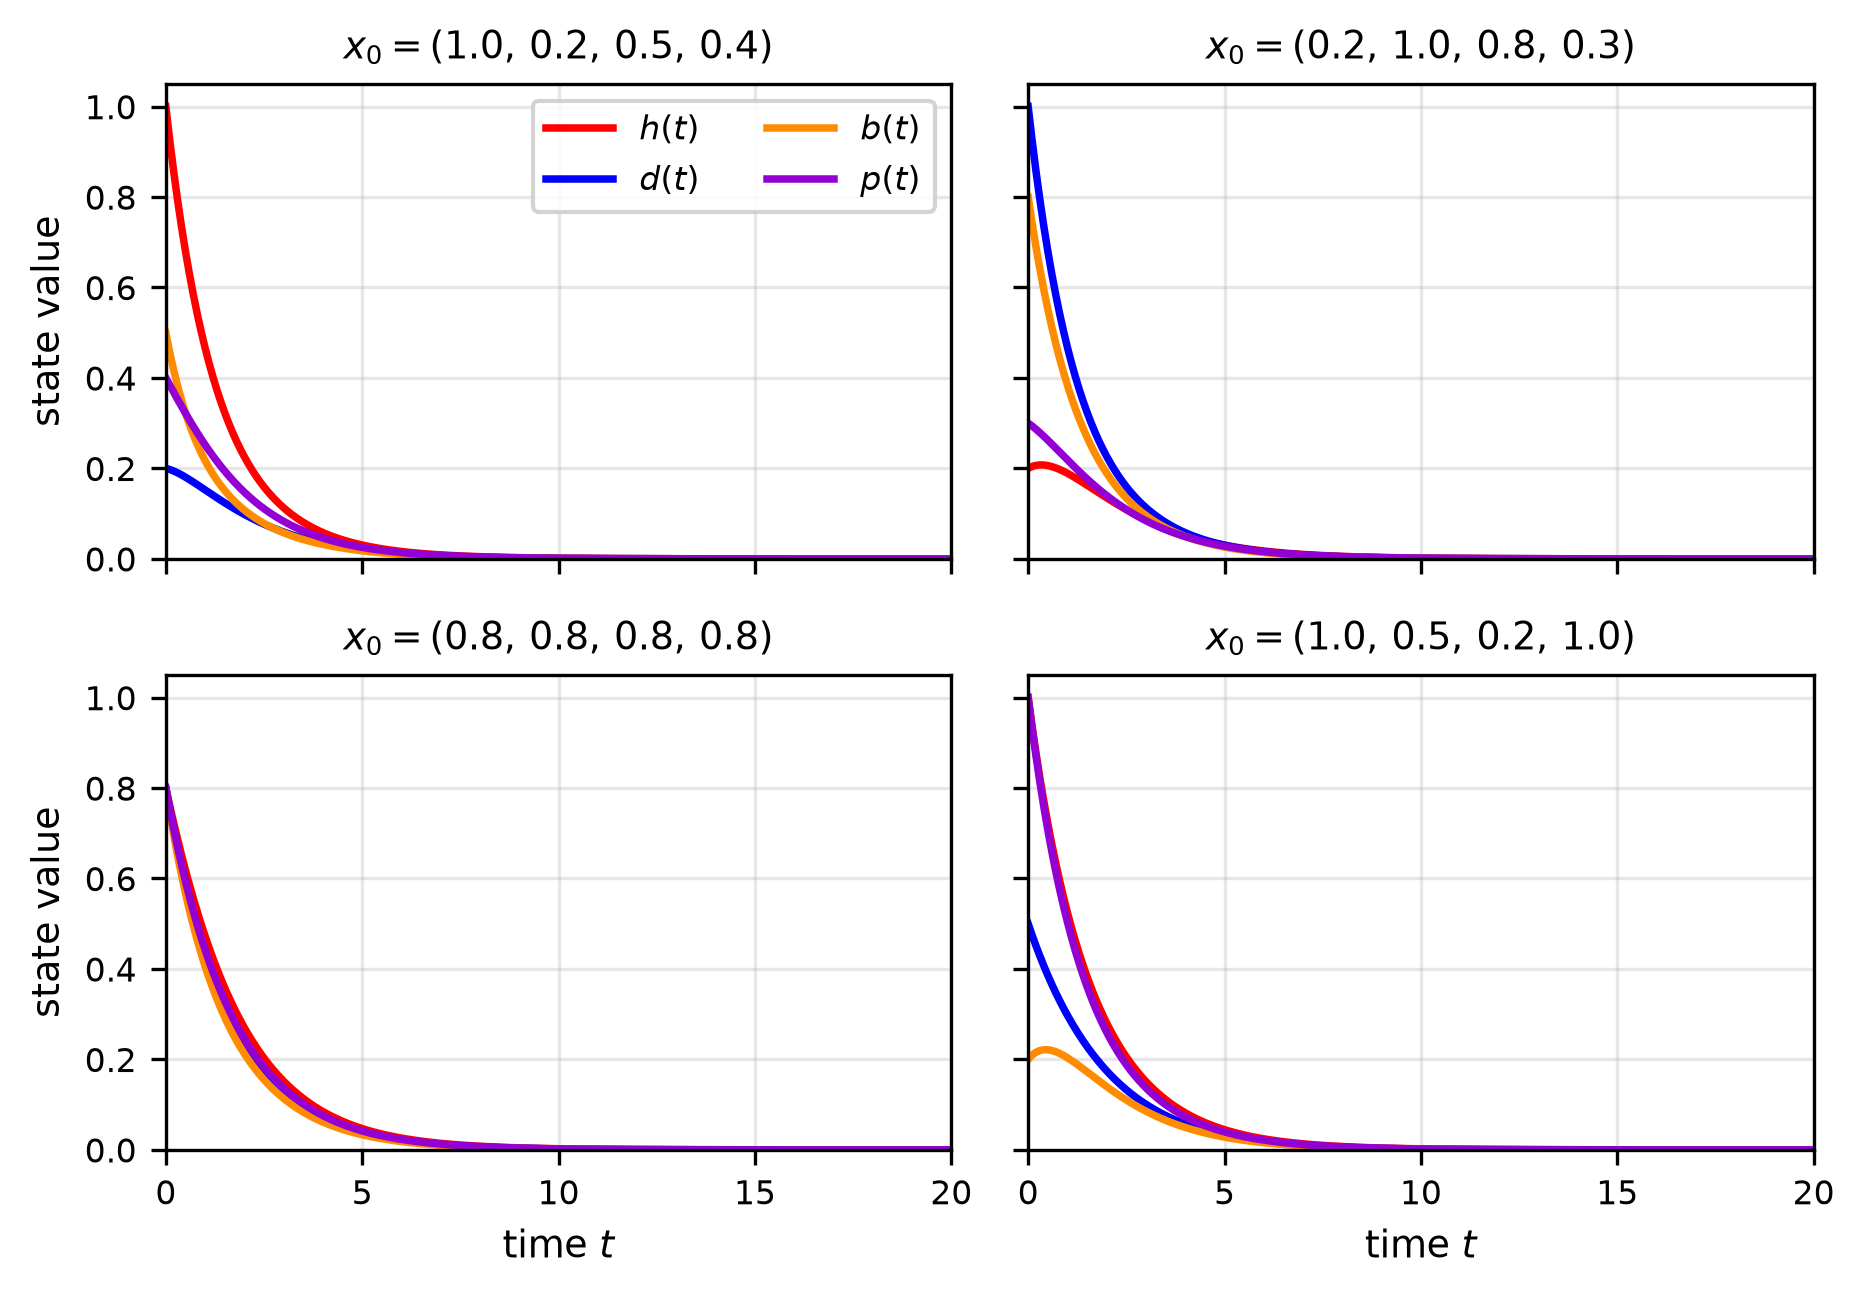
\includegraphics[width=\textwidth]{img/fig2_stable_trajectories.png}
\caption{Multi-panel simulation of the simplified energy poverty dynamics in a
stable regime ($\lambda_b=1.2>0$, all other parameters unchanged). All four state
variables converge to zero independently of initial conditions, indicating global
asymptotic stability.}
\label{fig:stable}
\end{figure}

In this regime, all eigenvalues of the system matrix have strictly negative real
parts; the dominant one is about $-0.598$ for the parameters used in
Figure~\ref{fig:stable}. The zero equilibrium is therefore globally
asymptotically stable, and all dimensions of deprivation converge to zero over
time, as the four panels show. Short-run oscillations may
occur due to complex eigenvalues, but they are damped and do not generate
persistent effects.

The qualitative difference between Figures~\ref{fig:unstable} and
\ref{fig:stable} highlights the critical role of direct energy-burden correction.
Once reinforcing feedback loops are counteracted by sufficiently strong
corrective mechanisms, the system no longer sustains energy poverty
endogenously.

From a policy perspective, the comparison between the two regimes illustrates
that reducing income poverty or arrears alone may be insufficient to eliminate
energy poverty. Without direct interventions targeting energy affordability,
feedback mechanisms may continue to reproduce deprivation. In contrast, policies
that structurally reduce energy burden break the feedback loop and ensure
convergence toward the non-deprived state.


\begin{comment}
\section{Policy Interpretation of Stability Conditions}

This section provides a practical interpretation of the stability conditions derived for the dynamical system of energy poverty. While the mathematical analysis shows that the zero equilibrium is asymptotically stable when the self-damping effects dominate the reinforcing cross-effects, it is equally important to understand what these inequalities mean in real social and policy terms. The following discussion translates the coefficients of the system into concrete mechanisms such as housing renovation, income support, debt management, and affordability measures, and explains how their relative strength determines whether energy poverty is gradually eliminated or persistently reproduced. In this way, the stability conditions are interpreted not only as mathematical criteria but also as guidelines for designing a policy system capable of driving the dynamics toward the desirable state of zero energy poverty.

The diagonal terms \(-\lambda_h\), \(-\lambda_d\), \(-\lambda_b\), and \(-\lambda_p\) represent the self-correcting mechanisms of the system. In practical terms, they correspond to policies or structural conditions that directly reduce each problem even without support from the other variables. For example:
\begin{itemize}
    \item \(\lambda_h\): renovation, insulation, efficient heating systems, emergency heating support,
    \item \(\lambda_d\): debt relief, arrears restructuring, disconnection protection,
    \item \(\lambda_b\): price caps, targeted subsidies, lower network charges, efficiency improvements,
    \item \(\lambda_p\): income support, minimum wages, social transfers, employment stability.
\end{itemize}

The off-diagonal coefficients, such as \(\alpha_{hb}\) and \(\alpha_{hp}\), represent reinforcing spillovers. For example:
\begin{itemize}
    \item high burden \(b\) worsens the inability to heat \(h\),
    \item poverty \(p\) increases arrears \(d\),
    \item arrears \(d\) worsen effective poverty \(p\),
    \item poor heating \(h\) may worsen health and indirectly affect income poverty.
\end{itemize}

Thus, the inequalities
\begin{align}
\lambda_h &> \alpha_{hb}+\alpha_{hp},\\
\lambda_d &> \alpha_{db}+\alpha_{dp},\\
\lambda_b &> \alpha_{bd}+\alpha_{bp},\\
\lambda_p &> \alpha_{pd}+\alpha_{ph}
\end{align}
This means that, for each dimension, the direct reduction capacity must exceed the total incoming reinforcing pressure from the other dimensions.



Under these inequalities, self-damping effects dominate reinforcing
cross-effects, and all deprivation dimensions converge to zero over time.

\paragraph{Interpretation.}
If the dominant eigenvalue is negative but close to zero, deprivation decays
very slowly. In this regime, households may remain trapped near a deprived
state for long periods, corresponding to a dynamic poverty trap. If the
dominant eigenvalue becomes positive, deprivation grows endogenously, and
energy poverty becomes self-sustaining in the absence of strong policy
intervention.

In practical terms, this means that energy poverty cannot be eliminated by addressing only one symptom. Instead, one needs a system in which, for every key mechanism:
\begin{itemize}
    \item the household receives enough direct support to reduce that specific deprivation, and
    \item the negative feedback loops from the other dimensions are weak enough not to recreate it.
\end{itemize}

For example, suppose a household receives an energy subsidy. This may reduce \(b\), the energy burden. But if income poverty \(p\) remains severe and arrears \(d\) continue to grow, then the subsidy alone may be too weak:
\[
\lambda_b \leq \alpha_{bd}+\alpha_{bp}.
\]
In that case, the burden is not structurally damped; it is continuously recreated by debt and poverty.

Hence, in practical policy terms, the inequalities imply that each domain must have enough policy strength to offset all the ways in which the other domains push households back into deprivation.

A realistic system leading to the zero equilibrium would combine at least four coordinated pillars.

\paragraph{1. Strong direct damping in each dimension.}
Each \(\lambda_i\) must be made sufficiently large. For example:
\begin{itemize}
    \item increase \(\lambda_h\) through deep renovation, insulation, heat pumps, replacement of inefficient boilers, and emergency winter aid,
    \item increase \(\lambda_d\) through debt counseling, regulated repayment plans, bans on punitive disconnection, and temporary debt forgiveness,
    \item increase \(\lambda_b\) through targeted tariff support, social tariffs, lower energy intensity of dwellings, and efficient appliances,
    \item increase \(\lambda_p\) through income support, rent support, labor-market inclusion, and broader anti-poverty policy.
\end{itemize}

\paragraph{2. Reduction of reinforcing cross-effects.}
Each \(\alpha_{ij}\) should be simplified where possible. For instance:
\begin{itemize}
    \item reduce \(\alpha_{bp}\): make poverty translate less strongly into high energy burden by subsidizing basic energy needs,
    \item reduce \(\alpha_{db}\): stop high burden from quickly turning into arrears via installment protections and bill smoothing,
    \item reduce \(\alpha_{ph}\): prevent inadequate heating from worsening poverty through health support and housing interventions,
    \item reduce \(\alpha_{hb}\): prevent cost burden from leading to underheating by guaranteeing a minimum energy service.
\end{itemize}

This is crucial: eliminating energy poverty is not only about increasing support but also about breaking the channels through which one deprivation creates another.

\paragraph{3. Early intervention.}
Even if the equilibrium is stable, large shocks may generate temporary hardship. Therefore, the system should detect rising risk before households fall into deep deprivation. This requires monitoring indicators such as:
\begin{itemize}
    \item rising share of income spent on energy,
    \item missed utility payments,
    \item self-reported inability to keep the home adequately warm,
    \item low income after housing and energy costs,
    \item poor building efficiency.
\end{itemize}
This helps prevent the state vector \(x(t)\) from moving too far away from zero.

\paragraph{4. Structural, not merely temporary, policy.}
If the diagonal damping comes only from temporary subsidies, stability may fail once the subsidy ends. A robust system, therefore, requires structural measures:
\begin{itemize}
    \item efficient housing stock,
    \item stable incomes,
    \item predictable energy pricing,
    \item consumer protections,
    \item accessible debt resolution.
\end{itemize}
Otherwise, the inequalities may hold only temporarily rather than permanently.

Recall, the mathematical statement that all trajectories converge to the origin if self-damping dominates reinforcing cross-effects translates into policy language as follows: energy poverty can be eradicated only if every mechanism that generates it is counteracted more strongly than it is reproduced by the rest of the social-energy system.

Thus, the goal is not merely to provide more subsidies but to build a system in which:
\begin{itemize}
    \item poor housing does not generate excessive costs,
    \item excessive costs do not generate arrears,
    \item arrears do not deepen poverty,
    \item poverty does not force underconsumption of energy.
\end{itemize}

This is precisely what the inequalities express.
%%%%%%%%%%%%%%%%%%%%%%%%new 
\end{comment}

%%%%%%%%%%%%%%%%%%


\section{Fuzzy Representation of Deprivation Dimensions}\label{sec:fuzzy}

The simplified system evolves on continuous deprivation intensities
$h(t)$, $d(t)$, $b(t)$, and $p(t)$. To connect these states with indicator-based
EU--SILC definitions, we introduce fuzzy membership functions. The operators,
transitions and indicators of this section are implemented in the module
\texttt{FuzzyEnergyPoverty.py} of the repository referenced in
Appendix~\ref{app:code}; all figures below are generated by that
implementation.

\paragraph{Fuzzy operators.}
We use the product t-norm
\[
x\otimes y = xy
\]
and the probabilistic sum
\[
x\oplus y = x+y-xy.
\]

\paragraph{Smooth thresholds.}
For $L<U$, we define cosine transitions
\begin{equation}\label{eq:costransition}
\Psi_{0\to1}(x;L,U)=
\begin{cases}
0,&x\le L,\\
\dfrac{1-\cos\!\left(\pi\dfrac{x-L}{U-L}\right)}{2},&L<x<U,\\
1,&x\ge U,
\end{cases}
\end{equation}
and analogously $\Psi_{1\to0}(x;L,U)$. Both functions are $C^1$-smooth and have a zero slope at $L$ and $U$.  Since the above transitions are intended to express gradual inequality, we will use relational notation for these mappings, as they are membership functions of binary fuzzy relations:
\begin{equation}\label{def:fuzzyineq}
(x\succeq_LU)=\Psi_{0\to1}(x;L,U)
\quad\text{and}\quad (x\preceq_LU)=\Psi_{1\to0}(x;L,U)
\end{equation}
we will explain in the subsequent sections.....
%%%%%%%%%%%%%%%%%%%

\subsection{Fuzzy Energy Poverty Indicators}

Each binary indicator in~\eqref{binary indicators new} is obtained by comparing a state variable with a crisp threshold. Replacing every such comparison by the corresponding gradual relation~\eqref{def:fuzzyineq}, conjunction by the t-norm $\otimes$ and disjunction by the t-conorm $\oplus$, we define
\begin{align}
\widetilde{I}_1(t)
&=
\bigl(h(t)\preceq_{L_h} U_h\bigr)
\oplus
\bigl(h(t)\succeq_{L_c} U_c\bigr),
&& \text{heating and cooling indicator},
\label{eq:index-heating-cooling}
\\[0.5em]
\widetilde{I}_2(t)
&=
\bigl(d(t)\succeq_{L_d} U_d\bigr),
&& \text{debt indicator},
\label{eq:index-debt}
\\[0.5em]
\widetilde{I}_3(t)
&=
\bigl(b(t)\succeq_{L_b} U_b\bigr)
\otimes
\underbrace{\bigl(y(t)\preceq_{L_p} U_p\bigr)}_{\mu_p(t)},
&& \text{energy expenses and income indicator},
\label{eq:index-expenses-income}
\end{align}
where \(y(t)\) denotes the income variable entering the poverty condition of~\eqref{binary indicators new} and \(\mu_p(t)\in[0,1]\) is the resulting degree of financial poverty.

In each case, the pair of thresholds brackets the crisp cut-off that it replaces,
\[
L_h\le\tau_h<U_h,\qquad
L_c<\tau_c<U_c,\qquad
L_d<\tau_d<U_d,\qquad
L_b<\tau_b<U_b,\qquad
L_p<\tau_p<U_p,
\]
and the transition width \(\Delta=U-L\) measures how much gradedness the definition admits. If every transition is centered at the corresponding crisp threshold, that is \(\tau=(L+U)/2\), then the symmetry of the cosine transition gives \(\Psi_{0\to1}(\tau;L,U)=\tfrac12\), so that thresholding a fuzzy indicator at the level \(\tfrac12\) reproduces exactly the original binary classification. Letting \(\Delta\to0\) in all transitions, \(\Psi_{0\to1}(x;L,U)\to\mathbf{1}\{x\ge\tau\}\) for every \(x\neq\tau\), the product t-norm reduces to conjunction and the probabilistic sum to disjunction. The binary indicators~\eqref{binary indicators new} are therefore recovered as a limiting case, and the fuzzy formulation is a proper generalization rather than a different measurement concept.

The cosine transitions are particularly suitable for this purpose because they are \(C^1\)-smooth and have zero derivatives at both endpoints. Hence, the indexes change continuously without abrupt jumps or sharp changes in slope when a state variable crosses one of the thresholds.

\begin{comment}
\paragraph{State-space form of the poverty membership.}
The poverty component of the dynamical system is the intensity \(p(t)\in[0,1]\), in which higher values correspond to more severe deprivation, whereas \(y(t)\) in~\eqref{eq:index-expenses-income} is an income variable, in which higher values correspond to less deprivation. Whenever the indicators are evaluated directly along the trajectories of the dynamical system, the same membership degree is therefore expressed as
\begin{equation}\label{eq:poverty-membership-state}
\mu_p(t)=\bigl(p(t)\succeq_{p_L}p_U\bigr),
\end{equation}
with \(p_L<p_U\) bracketing the intensity level at which the household is regarded as financially poor. Both variants are used below: the income form is convenient for interpretation in EU--SILC units, whereas~\eqref{eq:poverty-membership-state} keeps all three indicators as functions of the state vector \(x(t)=(h,d,b,p)^\top\) alone.

    
\paragraph{Thermal inadequacy as an intensity.}
The same distinction applies to the first indicator. If \(h(t)\) is measured as the indoor temperature, the two-sided form~\eqref{eq:index-heating-cooling} is required, because deprivation occurs at both ends of the temperature scale. If, as in the simplified dynamical system, \(h(t)\) is the intensity of thermal inadequacy, which already aggregates insufficient heating and insufficient cooling into a single deprivation-increasing variable, the indicator reduces to the one-sided form
\begin{equation}\label{eq:index-heating-intensity}
\widetilde I_1(t)=\bigl(h(t)\succeq_{L_h}U_h\bigr).
\end{equation}
The two readings are used consistently below: the temperature form in Section~\ref{sec:heating-cooling}, where the construction is illustrated in physical units, and the intensity form~\eqref{eq:index-heating-intensity} whenever the indicators are evaluated along trajectories of the dynamical system.
\end{comment}
%%%%%%%%%%%%%%%%%%%
\subsubsection{Debt Indicator}\label{sec:debt-indicator}
we start with this indicator because its simplicity.

The debt indicator~\eqref{eq:index-debt} replaces the crisp arrears condition \(\mathbf{1}\{d(t)\ge\tau_d\}\) by the gradual relation \(\bigl(d(t)\succeq_{L_d}U_d\bigr)\). In EU--SILC, arrears are recorded as a binary answer to the question whether the household was unable to pay utility bills on time during the preceding twelve months. The corresponding state variable \(d(t)\) of the dynamical system is, however, a continuous measure of accumulated payment difficulty. Depending on the level of aggregation, it may be interpreted as the amount of outstanding energy debt relative to monthly income, as the length of the payment delay, or as the prevalence of arrears within a population group. Below \(L_d\), payment delays are occasional and do not indicate financial distress; above \(U_d\), the household is unambiguously in arrears and exposed to enforcement or disconnection. Between the two thresholds, \(\widetilde I_2(t)\) expresses how far the process of indebtedness has advanced.

\begin{figure}[htbp]
\centering
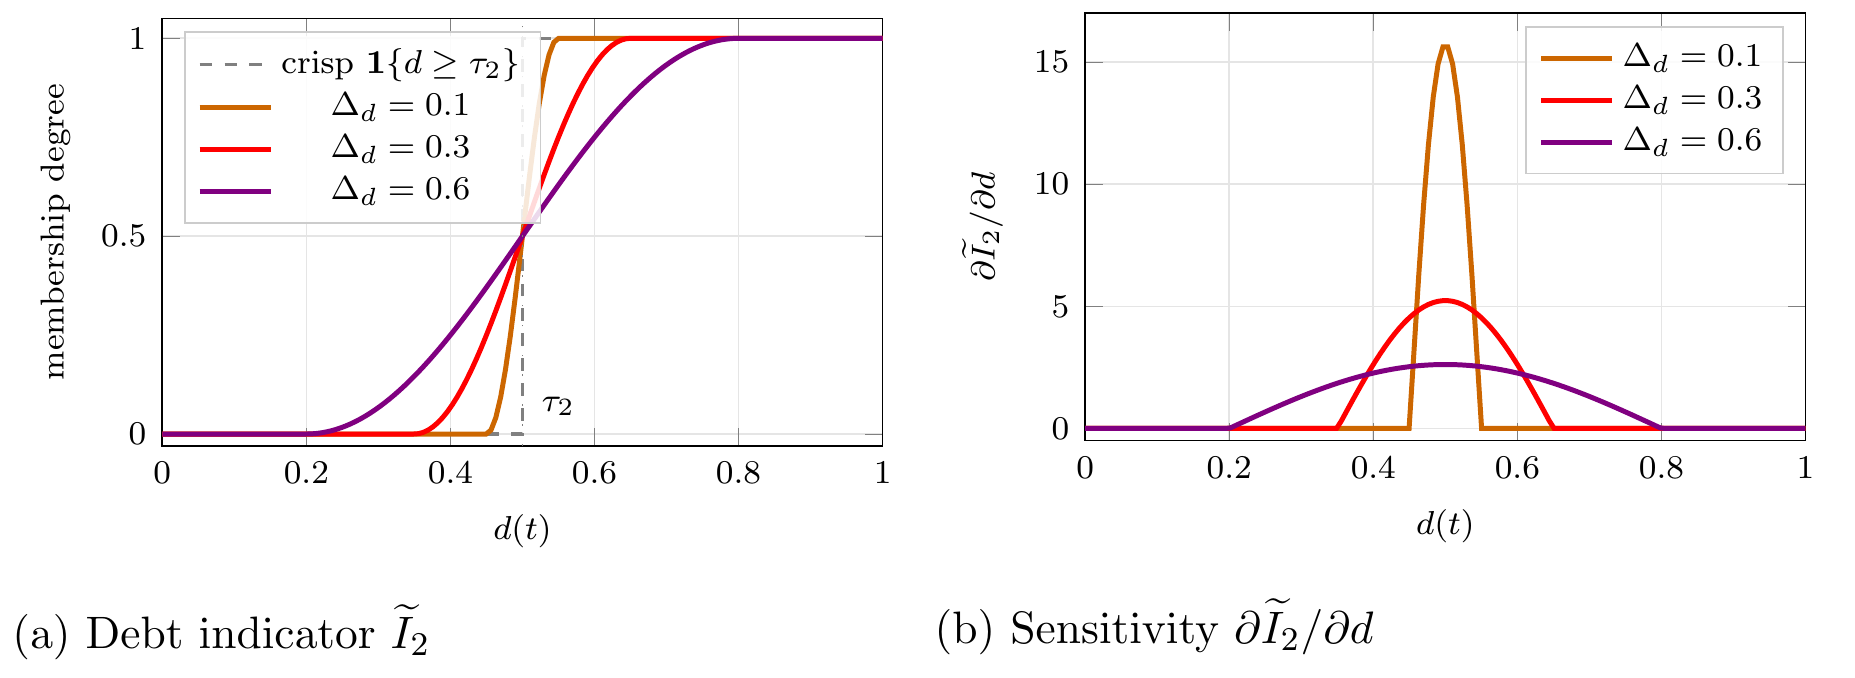
\includegraphics[width=\textwidth]{img/fig4_debt_indicator.png}
    \caption{Fuzzy debt indicator and its sensitivity for three transition widths
    $\Delta_d=U_d-L_d$ centered at the crisp threshold $\tau_d=0.5$. The dashed
    line in the left panel is the binary indicator obtained in the limit
    $\Delta_d\to0$.}
    \label{fig:debt-index}
\end{figure}

Figure~\ref{fig:debt-index}(a) shows the indicator for three transition widths centered at the same crisp threshold. All three curves pass through the value \(\tfrac12\) at \(d(t)=\tau_2\), so they classify households identically once a decision at level \(\tfrac12\) is required, while differing in how the intermediate region is described. Narrowing the interval moves the fuzzy indicator toward the binary step function, which is recovered in the limit \(\Delta_d\to0\).

The role of the transition width becomes explicit in the sensitivity of the indicator. Differentiating the cosine transition~\eqref{eq:costransition} gives
\begin{equation}\label{eq:dpsi}
\frac{\partial\widetilde I_2}{\partial d}
=
\Psi'_{0\to1}\bigl(d;L_d,U_d\bigr)
=
\begin{cases}
\dfrac{\pi}{2\Delta_d}\,
\sin\!\left(\pi\dfrac{d-L_d}{\Delta_d}\right), & L_d<d<U_d,\\[10pt]
0, & \text{otherwise},
\end{cases}
\end{equation}
which vanishes at both endpoints and attains its maximum \(\pi/(2\Delta_d)\) at the midpoint, as illustrated in Figure~\ref{fig:debt-index}(b). Consequently, a narrow transition concentrates the entire responsiveness of the indicator into a small neighborhood of the threshold and reproduces the instability of binary classification, in which negligible changes in arrears reverse the assessment. A wider transition distributes the responsiveness over a larger range of states and thus provides an early-warning signal before the administrative threshold is reached, at the cost of a weaker correspondence with the legal or statistical meaning of \(\tau_d\). In practice, \(\Delta_d\) should be chosen so that it reflects the measurement uncertainty of \(d(t)\) rather than being set arbitrarily.

Because \(\widetilde I_2\) is a smooth function of a single state variable, its evolution along a trajectory of the simplified system follows from the chain rule and~\eqref{eq:red_d},
\begin{equation}\label{eq:I2dot}
\frac{d}{dt}\widetilde I_2(t)
=
\Psi'_{0\to1}\bigl(d(t);L_d,U_d\bigr)\,\dot d(t)
=
\Psi'_{0\to1}\bigl(d(t);L_d,U_d\bigr)
\bigl(-\lambda_d d(t)+\alpha_{db}b(t)+\alpha_{dp}p(t)\bigr).
\end{equation}
The measured degree of deprivation therefore changes only for households whose arrears lie inside the transition band, and its rate of change is the product of a purely measurement-related factor and the dynamics generated by energy burden and poverty.


\subsubsection{Heating and Cooling Indicator}\label{sec:heating-cooling}

\begin{figure}[htbp]
\centering
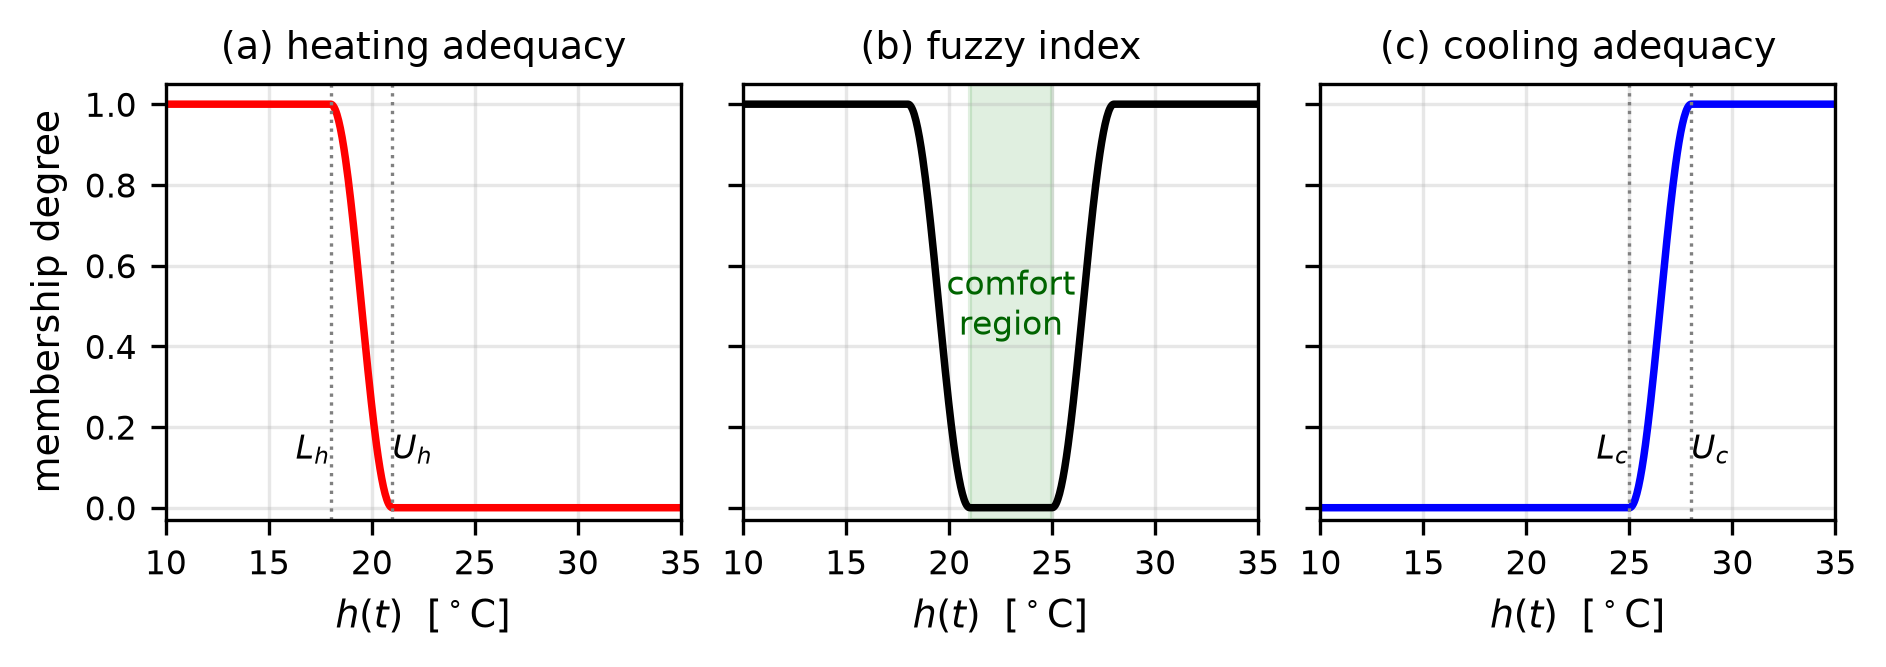
\includegraphics[width=\textwidth]{img/fig3_heating_cooling.png}
    \caption{Heating adequacy, the resulting fuzzy index, and cooling adequacy as functions of indoor temperature.}
    \label{fig:heating-cooling-index}
\end{figure}
Figure~\ref{fig:heating-cooling-index} illustrates the construction of the fuzzy heating-and-cooling indicator given by~\eqref{eq:index-heating-cooling}, where \(h(t)\) denotes the indoor temperature at time \(t\), the pair \(L_h<U_h\) delimits the transition associated with heating demand, and the pair \(L_c<U_c\) the transition associated with cooling demand. The first component describes the degree to which the indoor temperature is sufficiently low to indicate a need for heating, whereas the second component describes the degree to which it is sufficiently high to indicate a need for cooling.

The left panel shows the heating component. Two thresholds, denoted by \(L_h\) and \(U_h\), determine the transition interval. For temperatures \(h(t)\leq L_h\), the membership degree is equal to one, indicating a fully active heating demand. For temperatures \(h(t)\geq U_h\), the membership degree is zero, indicating that heating is not required. Between these thresholds, the membership degree decreases smoothly according to the cosine transition~\eqref{def:fuzzyineq}

The right panel represents the cooling component. Its transition is controlled by the thresholds \(L_c\) and \(U_c\). For temperatures \(h(t)\leq L_c\), the cooling membership degree is zero, since the indoor temperature is not sufficiently high to require cooling. For temperatures \(h(t)\geq U_c\), the membership degree is one, corresponding to a fully active cooling demand. Within the transition interval \((L_c,U_c)\), the cooling degree increases smoothly according to 
\(\Psi_{0\to 1}\bigl(h(t);L_c,U_c\bigr)
\)~\eqref{def:fuzzyineq}

The central panel shows the resulting fuzzy index obtained by aggregating the two components:
\[
\widetilde{I}_1(t)
=\bigl(h(t)\preceq_{L_h} U_h\bigr)
\oplus
\bigl(h(t)\succeq_{L_c} U_c\bigr).
\]
High values of \(\widetilde{I}_1(t)\) therefore indicate that either heating or cooling is needed. Conversely, low values correspond to the thermally adequate region in which neither component is substantially active.

The thresholds have a direct practical interpretation. The values \(L_h\) and \(U_h\) determine how gradually the assessment changes from a clear heating requirement to thermal adequacy. Similarly, \(L_c\) and \(U_c\) determine the transition from thermal adequacy to a clear cooling requirement. Increasing the width \(U_h-L_h\) or \(U_c-L_c\) produces a more gradual transition, whereas decreasing it makes the corresponding criterion closer to a crisp temperature threshold. In the illustrated specification, the cooling transition is placed at higher temperatures than the heating transition, creating an intermediate comfort region in which both membership degrees are close to zero.

%%%%%%%%%%%%%%%%%%%
\subsubsection{Energy Expenses and Income Indicator}\label{sec:expenses-income}

The third indicator differs from the previous two in that it is conjunctive: according to~\eqref{binary indicators new}, a household is deprived in this dimension only if a high share of energy expenditure occurs \emph{simultaneously} with low income. Its fuzzy counterpart~\eqref{eq:index-expenses-income} is accordingly the t-norm of two membership degrees,
\[
\widetilde I_3(t)=\mu_b(t)\otimes\mu_p(t)=\mu_b(t)\,\mu_p(t),
\qquad
\mu_b(t)=\bigl(b(t)\succeq_{L_b}U_b\bigr),
\qquad
\mu_p(t)=\bigl(y(t)\preceq_{L_p}U_p\bigr).
\]

\begin{figure}[htbp]
\centering
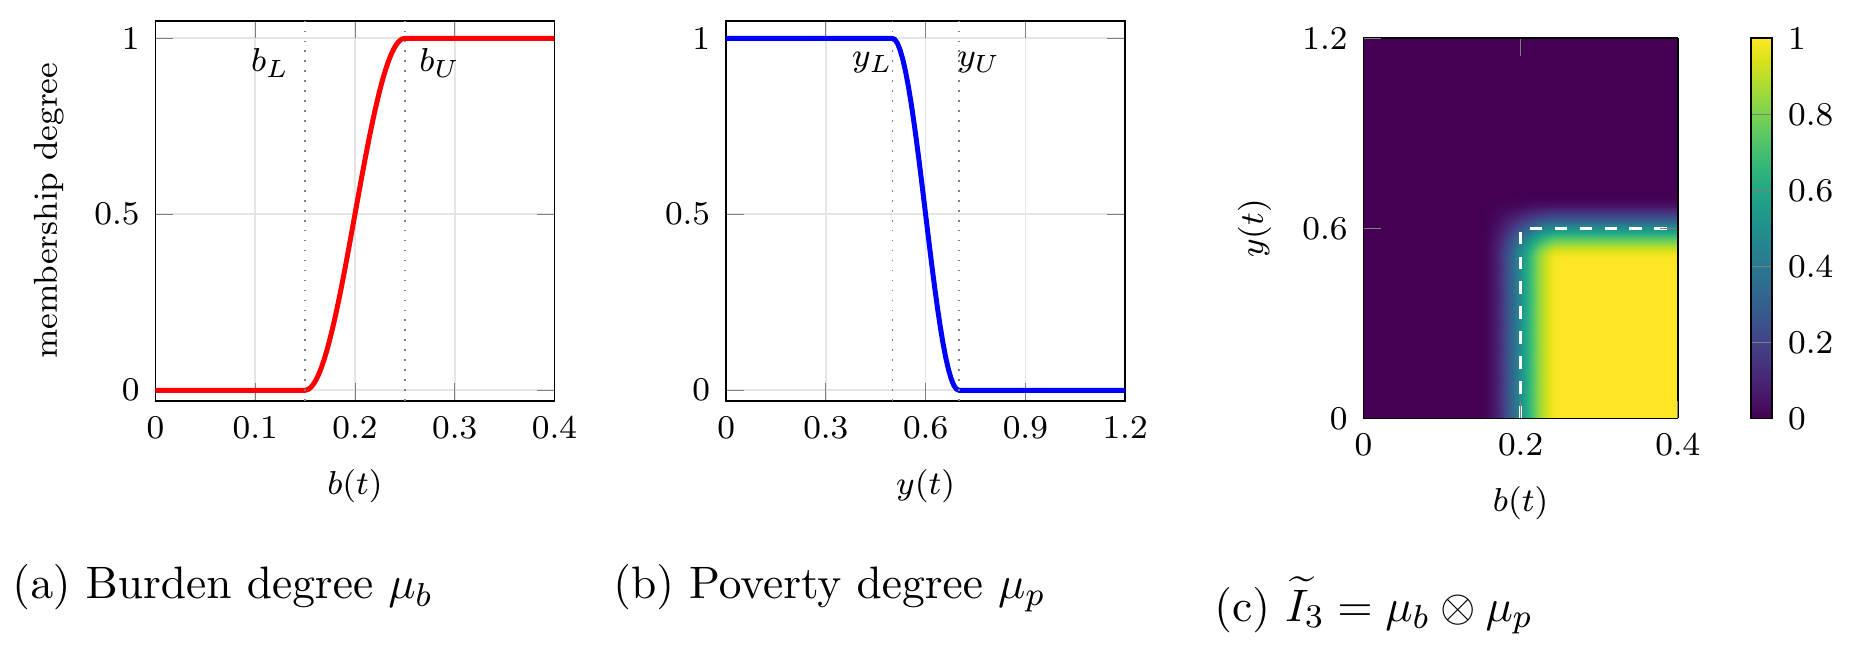
\includegraphics[width=\textwidth]{img/fig5_expenses_income.png}
    \caption{Construction of the fuzzy energy-expenses-and-income indicator with
    $L_b=0.15$, $U_b=0.25$ bracketing the burden threshold $\tau_d=0.20$, and
    $L_p=0.5$, $U_p=0.7$ bracketing the income threshold $\tau_p=0.6$ of the
    median residual income. The dashed line in panel~(c) delimits the crisp
    deprivation region $\{b\ge\tau_d\}\cap\{y\le\tau_p\}$ replaced by the
    graded one.}
    \label{fig:expenses-income-index}
\end{figure}

Figure~\ref{fig:expenses-income-index}(a) shows the burden component. The thresholds \(L_b\) and \(U_b\) are placed symmetrically around the national cut-off, here the Czech value \(\tau_d=0.20\) of the expenditure share; in another operationalization, the same construction applies with \(\tau_p\) given by twice the national median share used in the ``2M'' indicator, or by any other convention adopted in the country under study. Figure~\ref{fig:expenses-income-index}(b) shows the income component, in which the thresholds bracket the poverty line \(\tau_p=0.6\) of the median residual income. Since low income is the deprivation-increasing direction, the corresponding membership is decreasing.

Figure~\ref{fig:expenses-income-index}(c) displays the resulting indicator on the plane of the two arguments. The dashed line indicates the boundary of the crisp deprivation region that the fuzzy indicator replaces. The graded formulation smooths this boundary in both directions simultaneously, so that households situated near the corner \((\tau_d,\tau_p)\), which the binary definition separates sharply, receive intermediate degrees. 
{\color{red} write for all indices}


%%%%%%%%%%%%%%%%%%%
\subsection{Fuzzy Energy Poverty Index}

Let $w_1+w_2+w_3=1$, $w_i\ge0$. The fuzzy energy poverty index is defined as
\begin{equation}\label{eq:fuzzy-index}
\tilde P(t)=
w_1\tilde I_1(t)\oplus
w_2\tilde I_2(t)\oplus
w_3\tilde I_3(t).
\end{equation}
It is the gradual counterpart of the binary status $E_P(t)=\mathbf{1}\{I_1\lor I_2\lor I_3\}$, the disjunction being replaced by the t-conorm $\oplus$. Since $\oplus$ is monotone and $[0,1]$ is closed under it, $\tilde P(t)\in[0,1]$, and $\tilde P(t)$ increases whenever any of the three dimensions deteriorates. Note that the weights rescale the individual dimensions before aggregation, so that under equal weights $w_i=\tfrac13$ and full deprivation in all three dimensions the index attains $\tfrac13\oplus\tfrac13\oplus\tfrac13\approx0.704$ rather than one. The index should therefore be read as an ordinal measure of systemic stress; if a normalized scale is required, the weights must be chosen so that $\bigoplus_i w_i=1$.

\subsubsection{Behavior of the Index Along Trajectories}\label{sec:index-trajectories}

Because each fuzzy indicator is a smooth function of the state, the index evaluated along a solution of the simplified system, $\tilde P(t)=\tilde P(x(t))$, is differentiable and satisfies
\[
\frac{d}{dt}\tilde P(t)=\nabla\tilde P\bigl(x(t)\bigr)\cdot Ax(t).
\]
It therefore inherits the qualitative behavior established in Section~\ref{Analytical Solutions}: if all eigenvalues of $A$ have negative real parts, then $x(t)\to0$ and, since $\tilde P(0)=0$ at the origin, $\tilde P(t)\to0$; if $A$ has an eigenvalue with positive real part, the state does not converge to the origin and $\tilde P(t)$ remains bounded away from zero.

\begin{figure}[htbp]
\centering
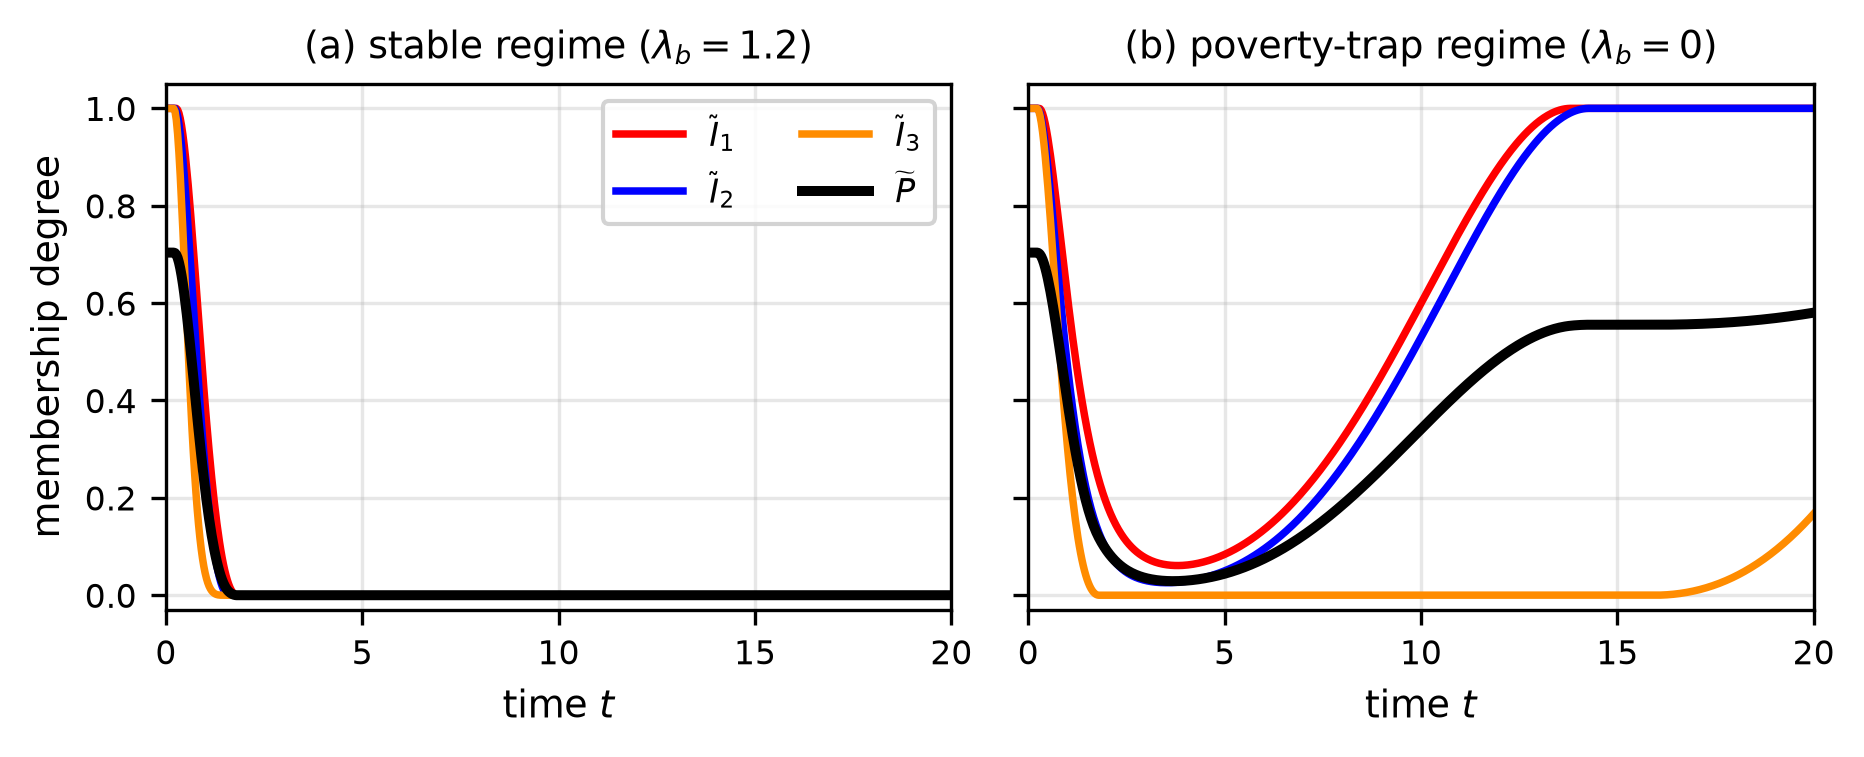
\includegraphics[width=\textwidth]{img/fig6_fuzzy_index.png}
    \caption{Fuzzy indicators and the composite index~\eqref{eq:fuzzy-index}
    along the trajectory starting from $x_0=(0.8,\,0.8,\,0.8,\,0.8)$ in the two
    regimes of Figures~\ref{fig:unstable} and~\ref{fig:stable}, with equal
    weights $w_i=\tfrac13$ and transitions $[0.3,0.7]$ in every dimension.}
    \label{fig:index-trajectory}
\end{figure}

Figure~\ref{fig:index-trajectory} illustrates both cases for the trajectory starting from full deprivation in all four dimensions. In the stable regime, Figure~\ref{fig:index-trajectory}(a), the indicators leave their saturation level in a definite order. The conjunctive indicator $\tilde I_3$ vanishes first, since it is a product of two memberships that both decrease, followed by the arrears indicator and finally by the thermal one; the whole index reaches zero within approximately two time units. Deprivation is thus eliminated endogenously once the energy burden is damped directly.

In the poverty-trap regime, Figure~\ref{fig:index-trajectory}(b), the picture is qualitatively different. The index first declines steeply, to $\tilde P\approx0.04$ around $t=3$, because the dimensions with positive self-correction recover quickly. The decline then stops and reverses, as the undamped energy burden feeds back through arrears and poverty. The dominant eigenvalue of the system matrix in this regime is approximately $0.075$, so deprivation grows slowly rather than explosively; the relapse appears first in the thermal and arrears components, which return to saturation by the end of the horizon, while $\tilde I_3$ begins to rise only at its very end. At $t=20$ the index has recovered to $\tilde P\approx0.58$ and keeps increasing. The comparison shows the practical value of a gradual measure: around $t=3$ the two regimes are nearly indistinguishable in terms of a binary classification, since almost no household would be recorded as energy poor, whereas the trajectory of $\tilde P$ separates a system that has been stabilized from one that is only temporarily improving before a relapse.

Because $\tilde P(t)$ is continuous and sensitive to intermediate levels of vulnerability, it can be used as an early-warning statistic rather than only as an ex-post classification. Its derivative is largest for households situated inside the transition bands, that is, precisely for those whose binary status is least stable.

%%%%%%%%%%%%%%%%%%%

\section{Empirical Illustration: the Role of $\lambda$ in Czech EU--SILC Data}
\label{sec:empirical-lambda}

The analysis so far has treated the self-correction rates $\lambda_h,\lambda_d,\lambda_b,\lambda_p$ as free parameters and shown, in Sections~\ref{sec:sim-trap} and~\ref{sec:sim-stable}, that the direct damping of the energy burden $\lambda_b$ is decisive for whether deprivation persists or fades. We now illustrate that this is not merely a theoretical possibility by calibrating the simplified system on Czech EU--SILC microdata and quantifying the empirical role of $\lambda$. The purpose is illustrative rather than predictive: with only two decades of annual observations the exercise cannot identify the full parameter set precisely, but it is sufficient to locate the observed system relative to the stability boundary and to see which of the four channels the margin of stability actually rests on.

\paragraph{Data and construction of the state series.}
We use household-level EU--SILC data for the Czech Republic covering 2005--2025, comprising roughly $8{,}500$ households per year. The memberships are built from the underlying continuous EU--SILC variables by the cosine transitions~\eqref{eq:costransition} of Section~\ref{sec:fuzzy}, not from the binary flags of the survey file, and are then averaged with the household cross-sectional weights to give a weighted annual prevalence for each dimension. Table~\ref{tab:silc-fuzzification} lists the variable and the pair of thresholds used for each state.

\begin{table}[htbp]
\centering
\small
\begin{tabular}{cllccc}
\toprule
\textbf{State} & \textbf{EU--SILC quantity} & \textbf{Membership} & $L$ & $U$ & $\tau$ \\
\midrule
$b$ & energy expenditure / net income & $\Psi_{0\to1}(\cdot;L_b,U_b)$ & $0.15$ & $0.25$ & $0.20$ \\
$p$ & residual income / poverty line & $\Psi_{1\to0}(\cdot;L_p,U_p)$ & $0.80$ & $1.20$ & $1$ \\
$d$ & arrears on utility bills & binary item & -- & -- & -- \\
$h$ & cannot keep the dwelling warm & binary item & -- & -- & -- \\
\bottomrule
\end{tabular}
\caption{Fuzzification of the four dimensions on EU--SILC microdata. Each pair
of thresholds is centred on the official cut-off $\tau=(L+U)/2$ it replaces --
the $20\,\%$ energy-burden cut-off and the at-risk-of-poverty line, the latter
recomputed for every year as $60\,\%$ of the weighted median residual income
per consumption unit -- so that thresholding a membership at $\tfrac12$
reproduces the official binary classification exactly, and the width
$\Delta=U-L$ is the only free parameter.}
\label{tab:silc-fuzzification}
\end{table}

Two remarks on this construction. First, the gradedness is genuine where the survey measures a quantity: $21\,\%$ of households fall strictly inside the burden band $(0.15,0.25)$ and $15\,\%$ strictly inside the poverty band $(0.8,1.2)$ around the line, so their membership is neither $0$ nor $1$ and their contribution to the annual prevalence is a fraction of a household rather than a whole one. Second, the gradedness is unavailable where the survey records only an answer: both the thermal item, ``the household cannot afford to keep the dwelling adequately warm'', and the arrears item, ``the household has been in arrears on utility bills'', are yes/no questions with no underlying continuous variable to compare against a threshold. For $h$ and $d$ the cosine transition therefore degenerates to the crisp indicator, which is the limiting case $\Delta\to0$ discussed after~\eqref{eq:costransition}. The fuzzy formulation is thus exercised exactly on the two dimensions the theory identifies as carrying the reinforcing feedback.

We identify the aggregate intensities with the state variables of the model, so that $h(t)$ is the thermal indicator $\tilde I_1$, $d(t)$ the debt indicator $\tilde I_2$, $b(t)$ the fuzzy energy-burden membership $\mu_b$, and $p(t)$ the fuzzy income-poverty membership $\mu_p$, each measured as a population share in $[0,1]$. The burden and poverty series are available from 2009 onward, giving $n=17$ annual points; they are shown in Figure~\ref{fig:empirical-lambda}(a). Income poverty is flat throughout, near $0.15$, while the energy burden is the most volatile dimension: it falls from $0.18$ in 2009 to $0.11$ in 2021 and rises again to $0.19$ in 2023, the year of the energy-price shock, which is also the year in which thermal deprivation doubles. Arrears are low and decline steadily.

\paragraph{Calibration.}
Interpreting the annual change of each series as a discrete approximation of its time derivative, we fit the simplified system~\eqref{eq:red_h}--\eqref{eq:red_p} with the sparsity pattern of the matrix $A$, adding a constant term that represents a persistent exogenous inflow and shifts the equilibrium away from the origin toward the observed levels. The model constrains the signs of the entries of $A$: every self-correction rate is non-negative and every cross-effect is non-negative, $\lambda_i\ge0$ and $\alpha_{ij}\ge0$. We impose that restriction in the estimation, so that the fitted matrix belongs to the class of matrices the theory is about; each equation is estimated by least squares subject to these bounds, and the self-correction rate of a dimension is read off the corresponding diagonal entry, $\lambda_i=-A_{ii}$. The estimated rates (per year) are
\[
\lambda_h\approx0.26,\qquad
\lambda_d\approx0.15,\qquad
\lambda_b\approx0.66,\qquad
\lambda_p\approx0.72,
\]
and the only cross-effects the data support with the sign the model requires are those acting on the burden equation, $\alpha_{bd}\approx2.12$ and $\alpha_{bp}\approx0.77$, together with a weak feedback of the burden on arrears, $\alpha_{db}\approx0.01$; the remaining cross-effects are estimated at the boundary, that is, at zero. The eigenvalues of the fitted $A$ are $-0.115$, $-0.259$, $-0.696$ and $-0.715$, all real and negative. The observed Czech system is therefore stable but only weakly so: deprivation returns to its equilibrium with a characteristic time of roughly $1/0.115\approx9$ years, which is the dynamical signature of a near-trap and is consistent with the well-documented persistence of energy poverty.

Unconstrained ordinary least squares does not stay inside the model class on these data. It returns a positive own-coefficient in the thermal equation, $\lambda_h\approx-0.34$, and four of the eight cross-effects with the sign opposite to the one the model assumes, which by itself makes the fitted matrix unstable, with dominant eigenvalue $\approx+0.35$. This is a statement about identification rather than about the Czech system: with sixteen annual differences, four coefficients per equation and series that rise and fall together, the unrestricted regression has little to separate a dimension's own persistence from the influence of its drivers. It is reported here because it fixes the accuracy the exercise can claim.

\begin{figure}[htbp]
\centering
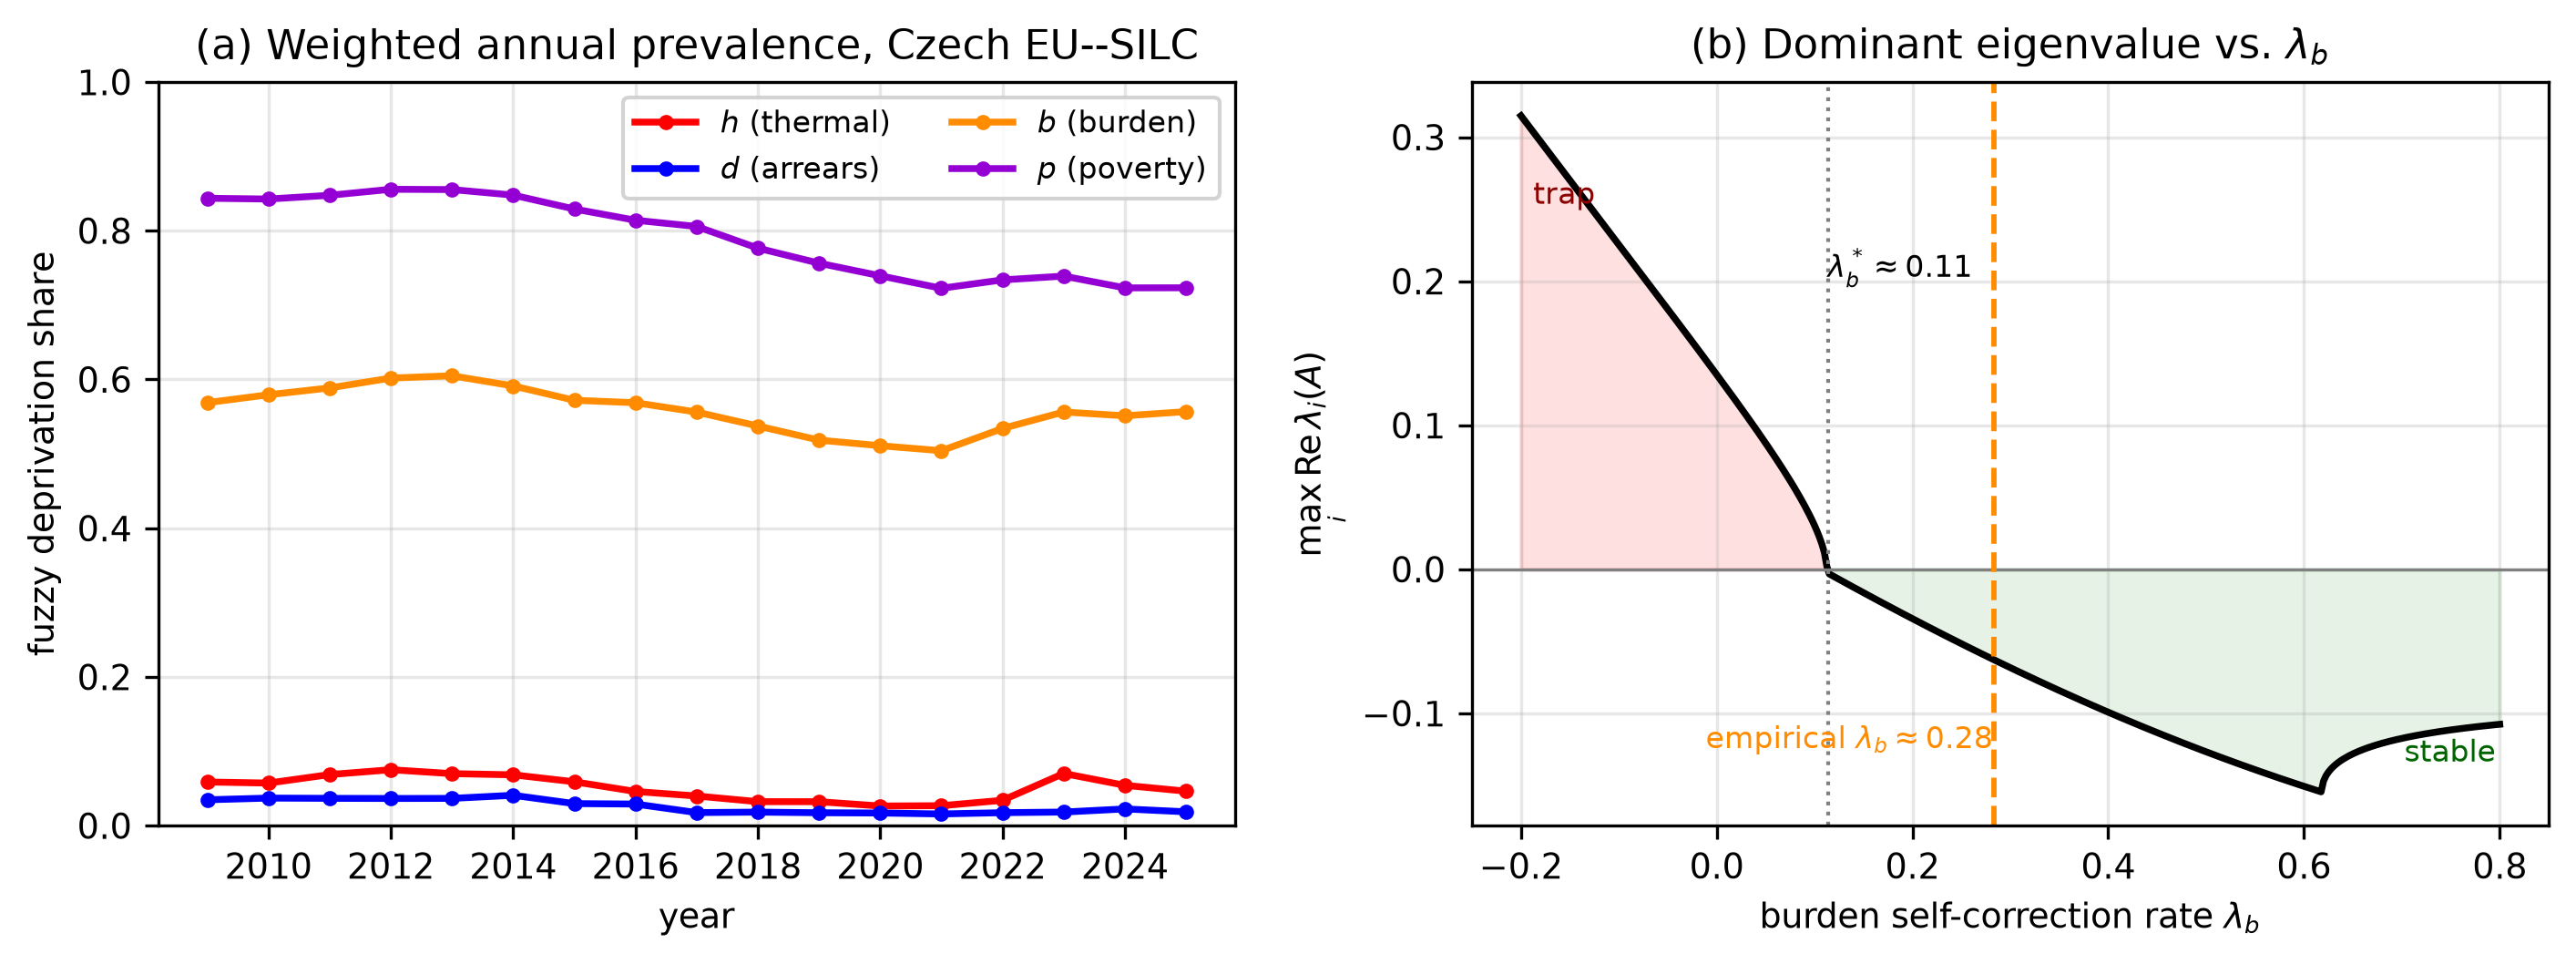
\includegraphics[width=\textwidth]{img/fig7_empirical_lambda.png}
\caption{Empirical role of the self-correction rate. (a) Weighted annual
prevalence of the four deprivation dimensions in Czech EU--SILC data,
2009--2025. (b) Dominant eigenvalue of the calibrated matrix $A$ as a function
of the burden self-correction rate $\lambda_b$, with the remaining parameters
fixed at their estimated values. The system is stable where the curve is
negative (green) and a poverty trap where it is positive (red); the crossing
defines the critical rate $\lambda_b^*\approx0.14$, while the estimated
$\lambda_b\approx0.66$ places the observed system on the stable side.}
\label{fig:empirical-lambda}
\end{figure}

\paragraph{Impact of $\lambda_b$.}
To isolate the role of the burden dimension we vary $\lambda_b$ while holding the remaining entries of $A$ at their estimated values and track the dominant eigenvalue, Figure~\ref{fig:empirical-lambda}(b). It decreases in $\lambda_b$ and changes sign at a critical value $\lambda_b^*\approx0.14$: below it the reinforcing feedback that reaches the burden from arrears and poverty overwhelms its own damping and the zero-deprivation equilibrium becomes unstable, whereas above it the system converges. The estimated $\lambda_b\approx0.66$ lies above this threshold by a factor of about five. The same sweep applied to $\lambda_h$ or $\lambda_p$ leaves the dominant eigenvalue negative for every positive rate, because in the fitted matrix nothing feeds back into those two dimensions; only $\lambda_d$ has a critical value of its own, $\lambda_d^*\approx0.03$. What the estimate therefore locates is not a single decisive rate but a single decisive loop: burden and arrears reinforce each other, and stability requires
\[
\lambda_b\lambda_d>\alpha_{bd}\alpha_{db}\approx0.021,
\]
which the estimated rates satisfy with $\lambda_b\lambda_d\approx0.101$. This is the empirical counterpart of the contrast between Figures~\ref{fig:unstable} and~\ref{fig:stable}: a structural weakening of energy-burden correction, for instance the withdrawal of affordability measures during a price shock, moves the real system toward $\lambda_b^*$, whereas policies that raise $\lambda_b$ enlarge the stability margin.

\paragraph{Robustness to the fuzzification.}
Because the thresholds of Table~\ref{tab:silc-fuzzification} are a modelling choice, the calibration is repeated for transition widths between $\Delta_b=0.002$ and $\Delta_b=0.20$, with $\Delta_p$ scaled accordingly. The estimates barely move: $\lambda_b$ stays within $[0.65,0.67]$, the dominant eigenvalue within $[-0.117,-0.111]$ and the critical rate within $[0.10,0.19]$, and the conclusion is unchanged in the near-crisp limit as well as when the arrears dimension is graded by the number of payment domains in arrears instead of the single utility item. The width of the transitions is thus not what drives the result; the choice of the underlying variable is. Substituting the survey file's own composite poverty score for income poverty, and its subjective housing-cost burden for the energy burden, moves the same estimator to $\lambda_b\approx0.42$ against a critical rate $\lambda_b^*\approx0.24$, that is, to a margin of stability roughly three times thinner, with a dominant eigenvalue of $-0.05$ instead of $-0.115$.

\paragraph{Caveats.}
The calibration gives an order of magnitude, not a precise estimate. Five limitations matter. First, the series are short: seventeen annual points carry little information about the coefficients. Second, averaging households into national shares hides the differences between them, so the model describes an average household rather than a varied population. Third, the equations are linear and closed, and therefore leave out the external forces—energy prices, weather, policy changes—that visibly move the observed series; the fit has to attribute their effect to the internal feedbacks. Fourth, the cross-effect coefficients are weakly identified, because the four series rise and fall together and the regression cannot cleanly separate their mutual influences; five of the eight are estimated at the boundary of the admissible sign region, and the unconstrained fit leaves that region altogether. Fifth, two of the four dimensions are measured by binary survey items, so the gradual measure is exercised on the burden and poverty dimensions only.

One conclusion nevertheless survives, because it is qualitative rather than numerical. The reinforcing feedback that the data support runs through the energy burden: it is the only equation whose drivers are estimated away from zero, and the stability of the fitted system is decided by the loop it forms with arrears. That is the channel the theory of Sections~\ref{sec:sim-trap} and~\ref{sec:sim-stable} singles out in advance. The data were free to place the reinforcement elsewhere and did not. The exercise therefore supports the mechanism developed above, even though it cannot measure it.

%%%%%%%%%%%%%%%%%%%


\appendix
\section{Reproducibility and Source Code}\label{app:code}

Every figure in this paper is generated from the model itself rather than drawn
by hand, and the numerical values quoted in the text can be recomputed from the
same source. The complete implementation is openly available in the repository
\begin{center}
\url{\codeurl}
\end{center}
and consists of four Python modules. The module \texttt{FuzzyEnergyPoverty.py}
implements the fuzzy layer of Section~\ref{sec:fuzzy}: the product t-norm, the
probabilistic sum, the cosine transitions~\eqref{eq:costransition} together with
their derivative~\eqref{eq:dpsi}, the three indicators, and the composite
index~\eqref{eq:fuzzy-index}. The script \texttt{paper\_figures.py} integrates
the simplified system~\eqref{eq:red_h}--\eqref{eq:red_p} and draws all figures,
collecting every parameter that appears in a caption in a single configuration
block; running it reproduces the figures of this paper together with the
eigenvalues and index levels quoted in the text. The module
\texttt{silc\_fuzzy.py} builds the household-level memberships of
Table~\ref{tab:silc-fuzzification} from the raw EU--SILC variables of the file
\texttt{dom\_all\_echudoba.RDS}: it recomputes the yearly at-risk-of-poverty
line, applies the cosine transitions~\eqref{eq:costransition} to the energy
expenditure share and to the relative residual income, collects all threshold
parameters in a single dataclass, and reports how much of the population falls
strictly inside each transition band and whether the $\tfrac12$-cut of every
membership reproduces the official binary classification. The script
\texttt{empirical\_lambda.py} carries out the empirical calibration of
Section~\ref{sec:empirical-lambda}: it builds the weighted annual prevalence
series, estimates the self-correction rates $\lambda_i$ under the sign
restrictions of the model as well as by unconstrained least squares, repeats the
estimation for the alternative transition widths of the robustness check, and
produces Figure~\ref{fig:empirical-lambda} together with the eigenvalues and the
critical rate $\lambda_b^*$ quoted in the text.
Table~\ref{tab:code-map} maps the figures to the functions that produce them.

\begin{table}[h!]
\centering
\small
\begin{tabular}{llll}
\toprule
\textbf{Output} & \textbf{Section} & \textbf{Function in \texttt{paper\_figures.py}} \\
\midrule
Figure~\ref{fig:unstable} & \ref{sec:sim-trap} & \texttt{figure\_trajectories("trap", \ldots)} \\
Figure~\ref{fig:stable} & \ref{sec:sim-stable} & \texttt{figure\_trajectories("stable", \ldots)} \\
Figure~\ref{fig:heating-cooling-index} & \ref{sec:heating-cooling} & \texttt{figure\_heating\_cooling()} \\
Figure~\ref{fig:debt-index} & \ref{sec:debt-indicator} & \texttt{figure\_debt()} \\
Figure~\ref{fig:expenses-income-index} & \ref{sec:expenses-income} & \texttt{figure\_expenses\_income()} \\
Figure~\ref{fig:index-trajectory} & \ref{sec:index-trajectories} & \texttt{figure\_fuzzy\_index()} \\
Eigenvalues and index levels & \ref{sec:sim}, \ref{sec:index-trajectories} & \texttt{report()} \\
Figure~\ref{fig:empirical-lambda} & \ref{sec:empirical-lambda} & \texttt{empirical\_lambda.py} (\texttt{main}) \\
\bottomrule
\end{tabular}
\caption{Correspondence between the figures of the paper and the code.}
\label{tab:code-map}
\end{table}


\bibliographystyle{abbrv}
\bibliography{references}
\end{document}
